%----------------------------------------------------------------------------------------
%	PACKAGES AND THEMES
%----------------------------------------------------------------------------------------
\documentclass[aspectratio=169,xcolor=dvipsnames]{beamer}
\usetheme{SimplePlus}

\usepackage{hyperref}
\usepackage{graphicx} % Allows including images
\usepackage{booktabs} % Allows the use of \toprule, \midrule and \bottomrule in tables
\setbeamerfont{block title}{size=\Huge}

\setbeamerfont{block body}{size=\Huge}

%----------------------------------------------------------------------------------------
%	TITLE PAGE
%----------------------------------------------------------------------------------------

\title[short title]{Spurious Solar-Wind Effects on Acceleration Noise in LISA Pathfinder
} % The short title appears at the bottom of every slide, the full title is only on the title page

\author{Indie Desiderio-Sloane and Arnold Yang}

\institute[Institute for Computing in Research] % Your institution as it will appear on the bottom of every slide, may be shorthand to save space
{
   Institute for Computing in Research
}
\date{\today} % Date, can be changed to a custom date


%----------------------------------------------------------------------------------------
%	PRESENTATION SLIDES
%----------------------------------------------------------------------------------------

\begin{document}

\begin{frame}
    % Print the title page as the first slide
    \titlepage
\end{frame}
\iffalse
%------------------------------------------------
\begin{frame}{Sir Isaac Newton}
    \centering
    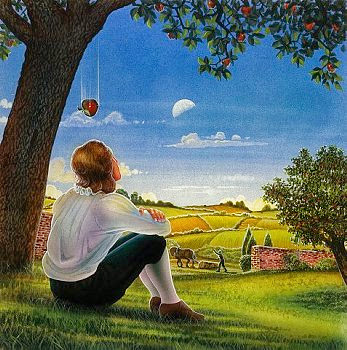
\includegraphics[height=7cm]{newton.jpg}\\
    \scalebox{.4}{ https://briankoberlein.com/post/newtons-apple/}
\end{frame}
\fi
\iffalse 
%------------------------------------------------
\begin{frame}{Oliver Heaviside \& Henry Poincare}
 \begin{columns}[t]
    \begin{column}{3cm}
    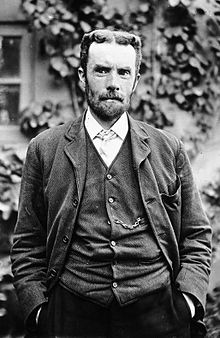
\includegraphics[height=6cm]{220px-Oheaviside.jpg}
    \scalebox{.4}{https://en.wikipedia.org/wiki/Oliver\_Heaviside}
    \end{column}
    \begin{column}{6cm}
    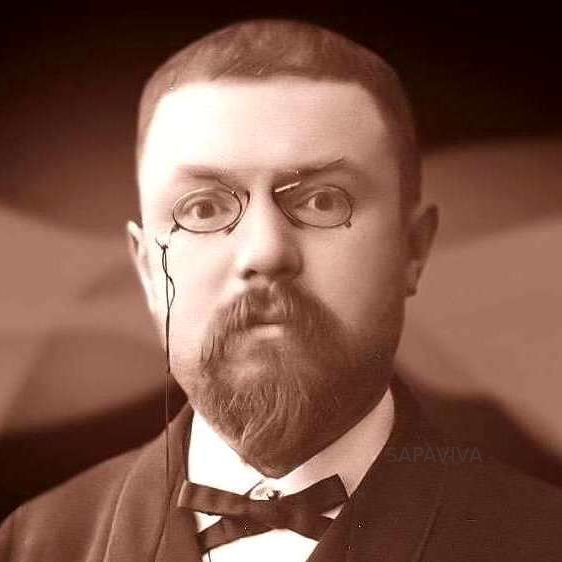
\includegraphics[height=6cm]{henry.jpg}
    \scalebox{.4}{ https://www.sapaviva.com/jules-henri-poincare/}
    \end{column}
\end{columns}
\end{frame}
%------------------------------------------------
\fi
\begin{frame}{Albert Einstein}
    %\centering
    \begin{columns}[t]
    \begin{column}{4cm}

    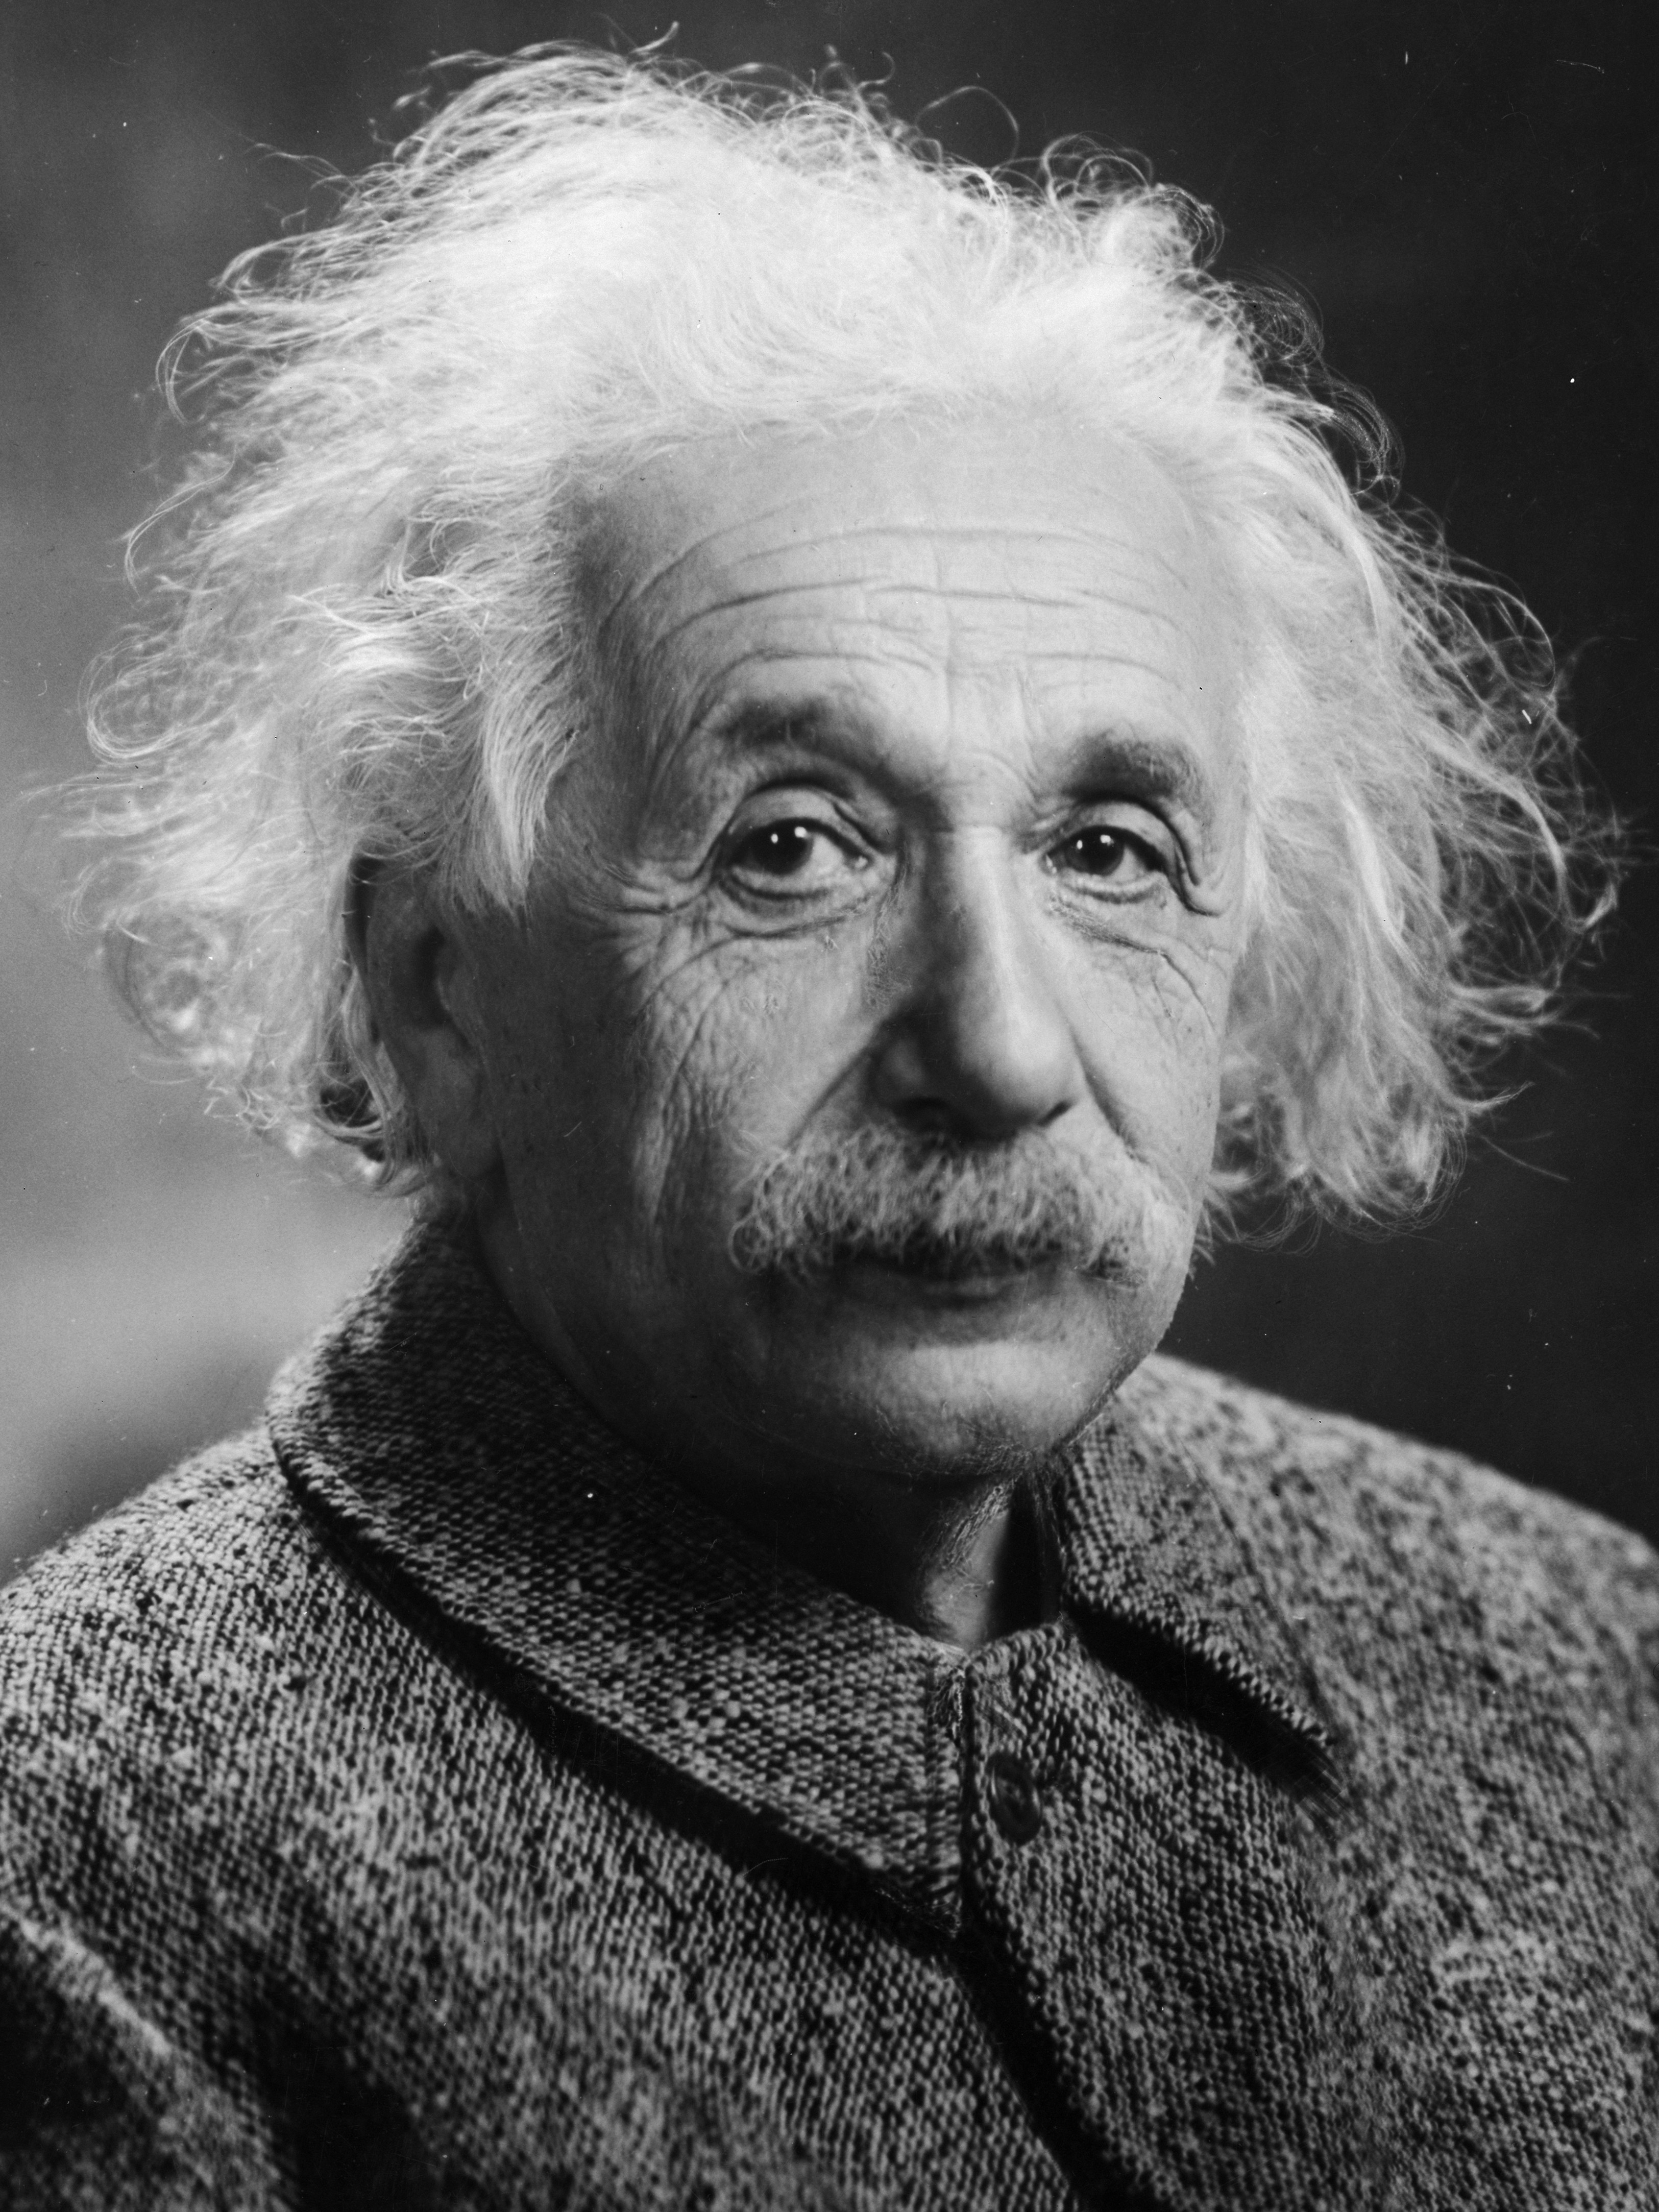
\includegraphics[height=6cm]{einstein.jpg}
    \scalebox{.4}{ https://commons.wikimedia.org/wiki/File:Albert\_Einstein\_Head.jpg}
    \end{column}
    \begin{column}{7cm}


    \begin{varblock}
    \vspace{1cm}
    \Huge\[G_{\mu\nu}=\frac{8\pi G}{c{^4}}T_{\mu\nu}\]
    \end{varblock}
   % 
   %% \begin{varblock}
   % \Huge\[h=\frac{2G}{c{^4}}\frac{1}{r}\frac{\delta{^2}Q}{\delta t{^2}}\]
   % \end{varblock}
    \end{column}
    \end{columns}
     
\end{frame}
\iffalse
%------------------------------------------------
\begin{frame}{Albert Einstein}
    %\centering
    \begin{columns}[t]
    \begin{column}{4cm}

    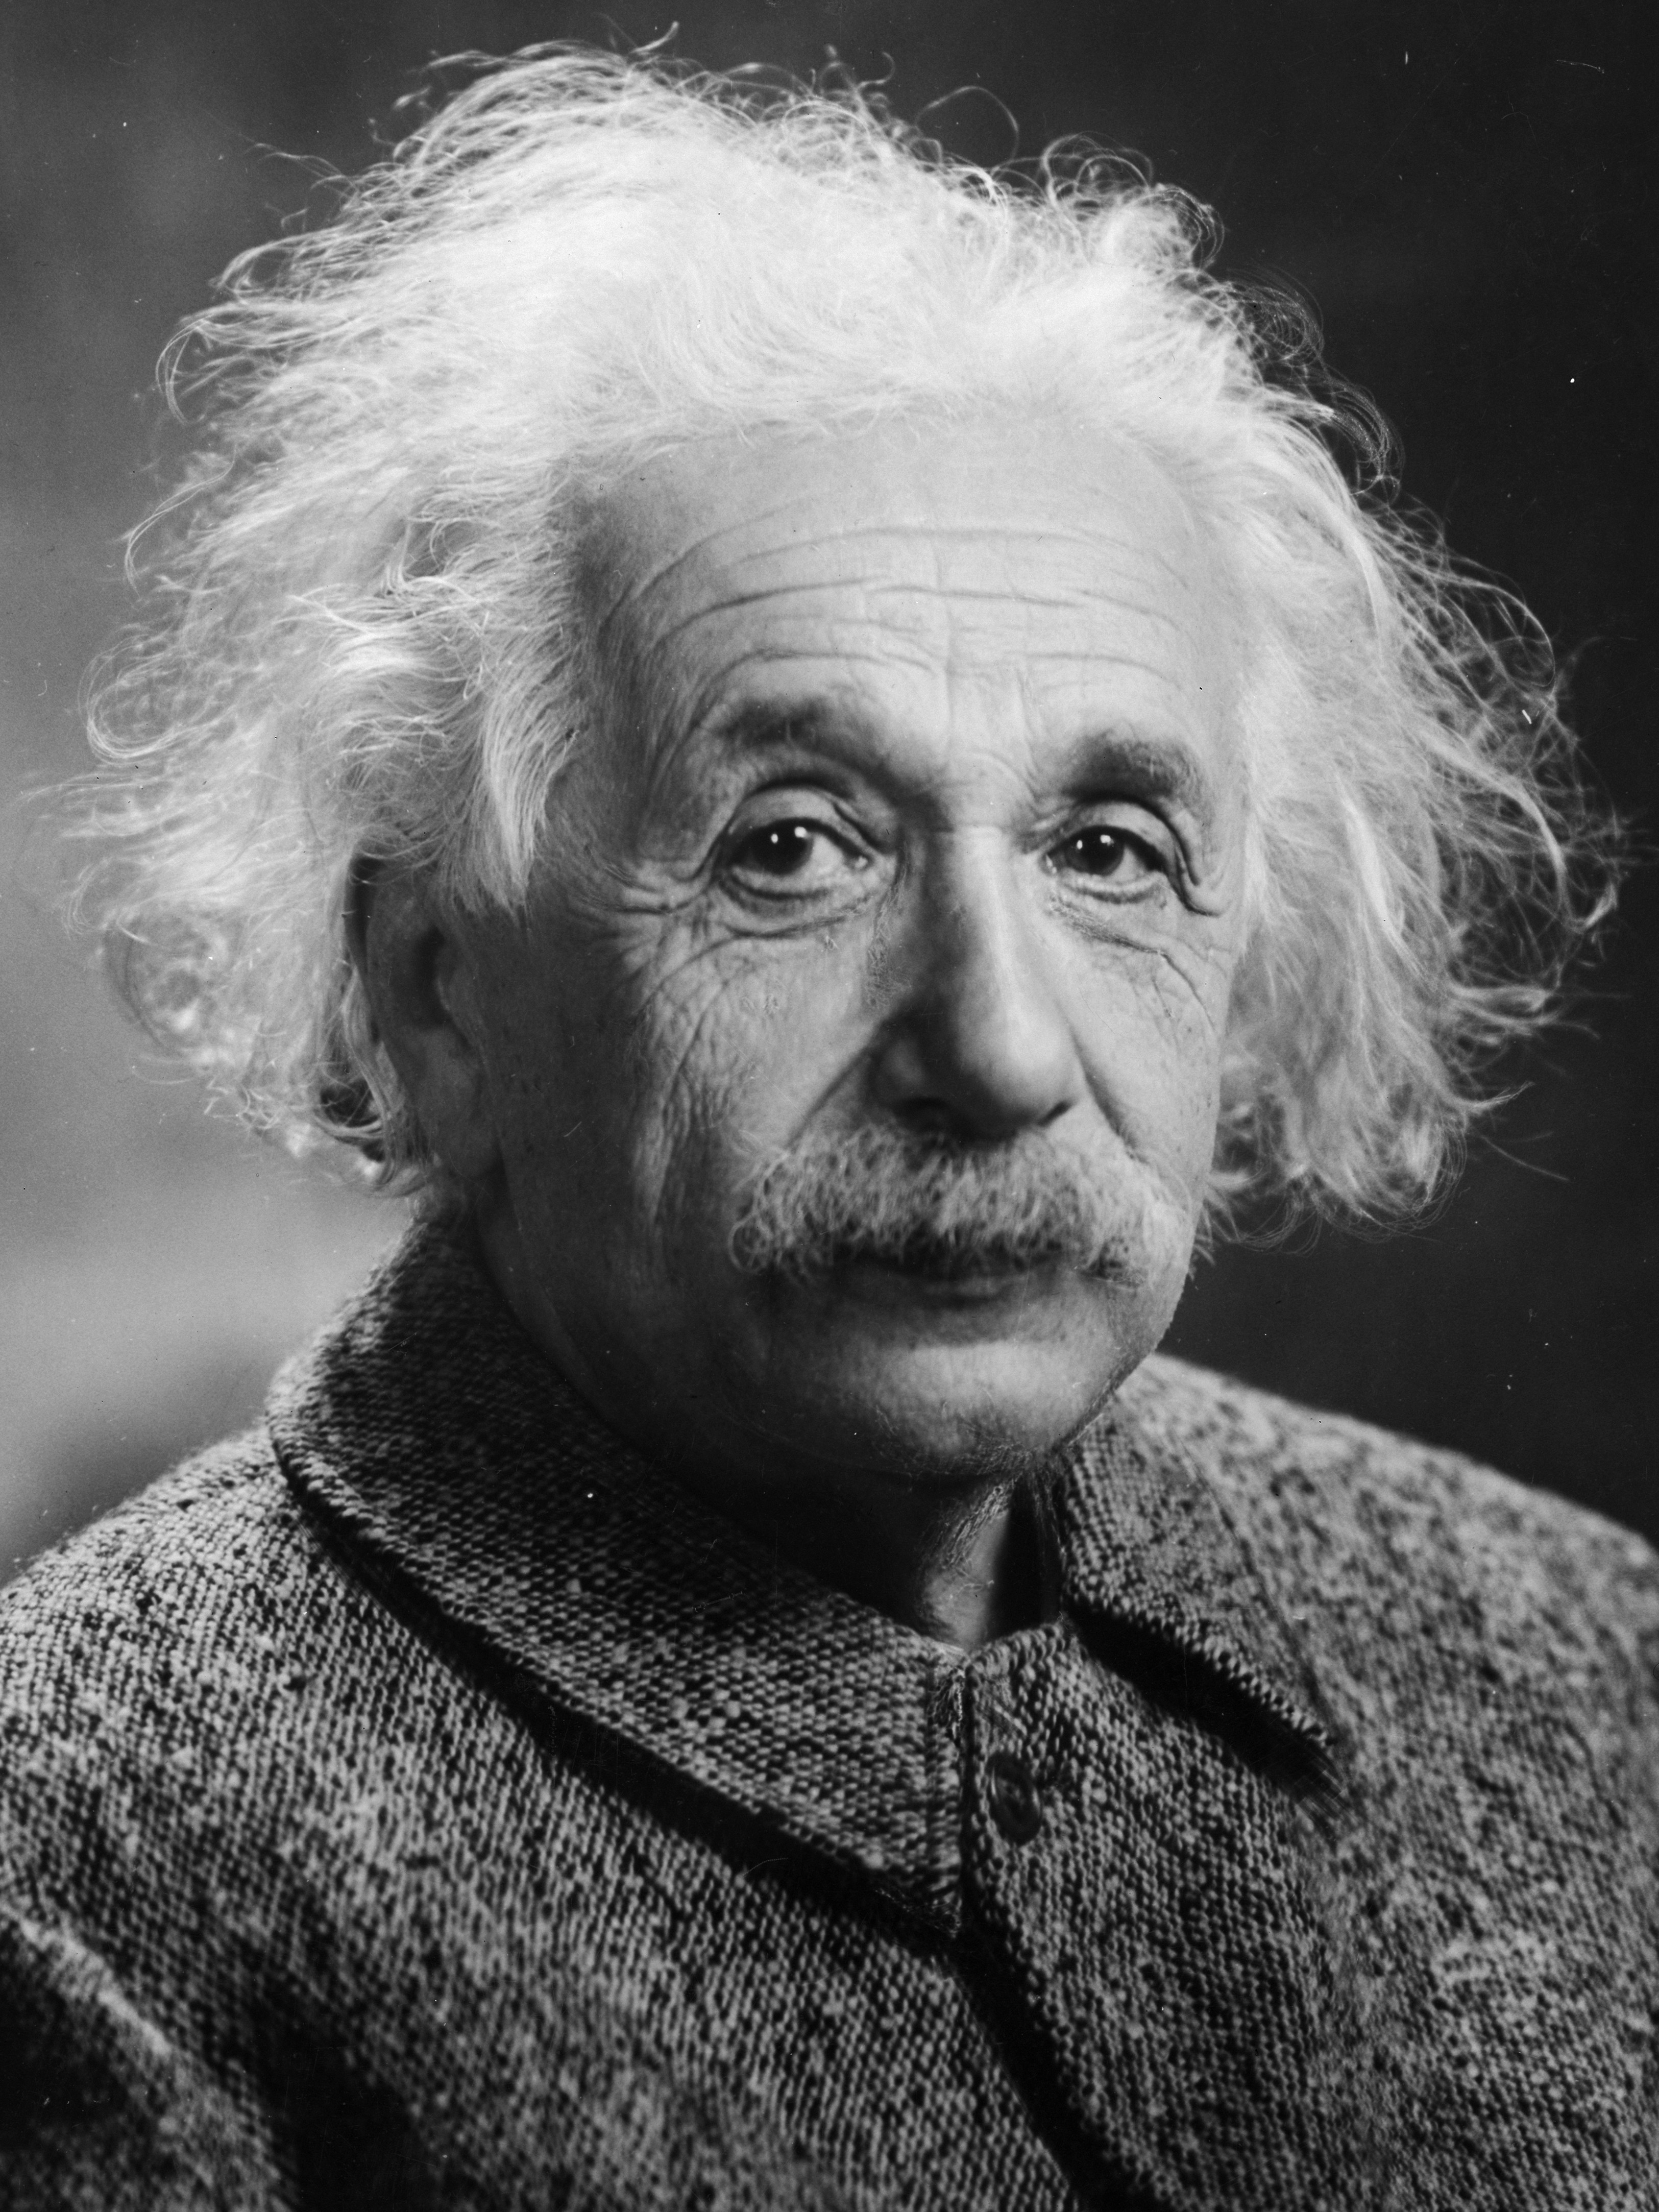
\includegraphics[height=6cm]{einstein.jpg}
    \scalebox{.4}{ https://commons.wikimedia.org/wiki/File:Albert\_Einstein\_Head.jpg}
    \end{column}
    \begin{column}{7cm}


  
    \begin{varblock}
    \\
    \textit{"Since then [November 14] I have handled Newton’s case differently, of course, according to the final theory [the theory of General Relativity]. Thus there are no gravitational waves analogous to light waves. This probably is also related to the one-sidedness of the sign of the scalar T, incidentally [this implies the nonexistence of a “gravitational dipole"].}
    \\
    \vspace{2cm}
    --Albert Einstein, letter to Swarzchild 1916
   % \Huge\[h=\frac{2G}{c{^4}}\frac{1}{r}\frac{\delta{^2}Q}{\delta t{^2}}\]
    \end{varblock}
    \end{column}
    \end{columns}
     
\end{frame}
%---------------------------------------------
\begin{frame}{Arthur Eddington}
    %\centering
    \begin{columns}[t]
    \begin{column}{4cm}

    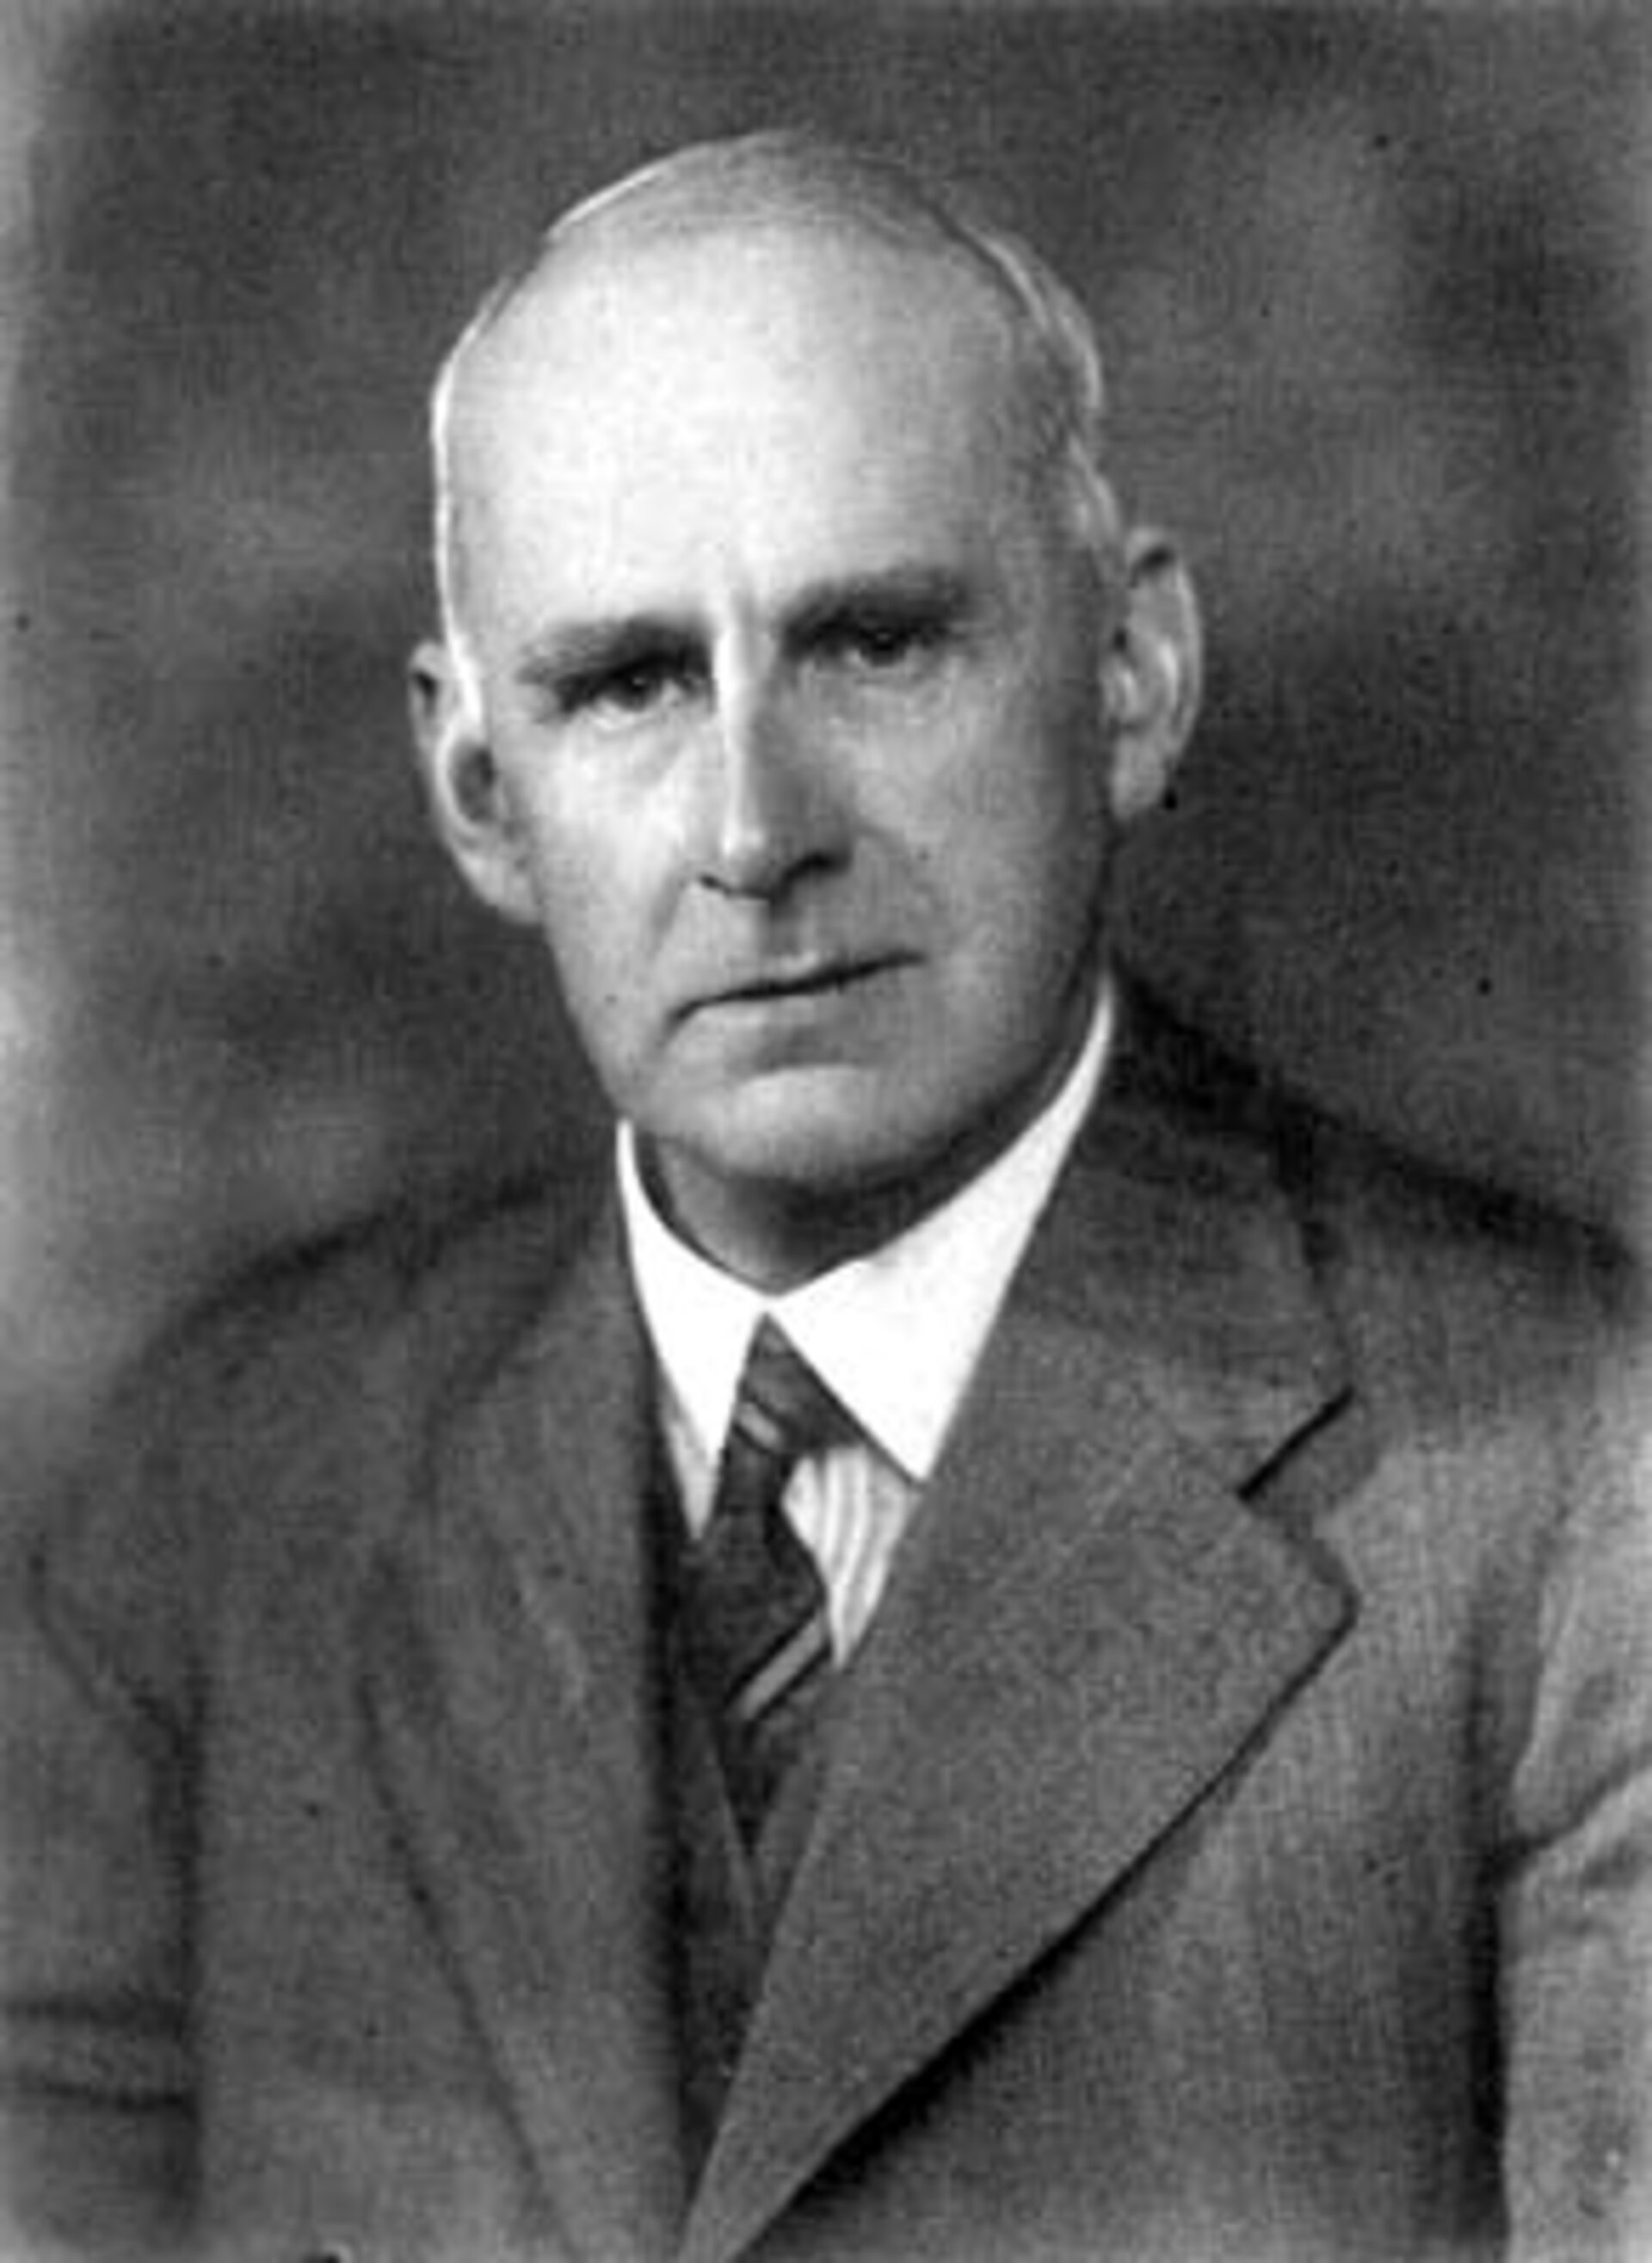
\includegraphics[height=6cm]{Arthur_Stanley_Eddington_1882_-_1944_pillars.jpg}
    \scalebox{.4}{https://www.esa.int/var/esa/storage/images/esa\_multimedia/images/2003/07/arthur\_stanley\_eddington\_1882\_-\_1944/9583215-3-eng-GB/Arthur\_Stanley\_Eddington\_1882\_-\_1944\_pillars.jpg}
    \scalebox{.4}{https://www.bbvaopenmind.com/wp-content/uploads/2019/05/Eddington-3-1-1.jpg}
    \end{column}
    \begin{column}{8cm}

    \begin{varblock}
    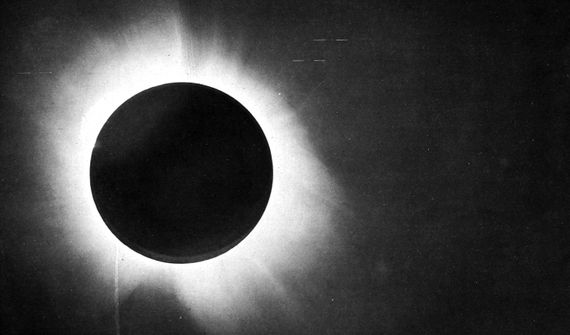
\includegraphics[height=4cm]{Eddington-3-1-1.jpg}
   % \Huge\[h=\frac{2G}{c{^4}}\frac{1}{r}\frac{\delta{^2}Q}{\delta t{^2}}\]
    \end{varblock}
    \end{column}
    \end{columns}
     
\end{frame}

%---------------------------------------------
\begin{frame}{Arthur Eddington}
    %\centering
    \begin{columns}[t]
    \begin{column}{4cm}

    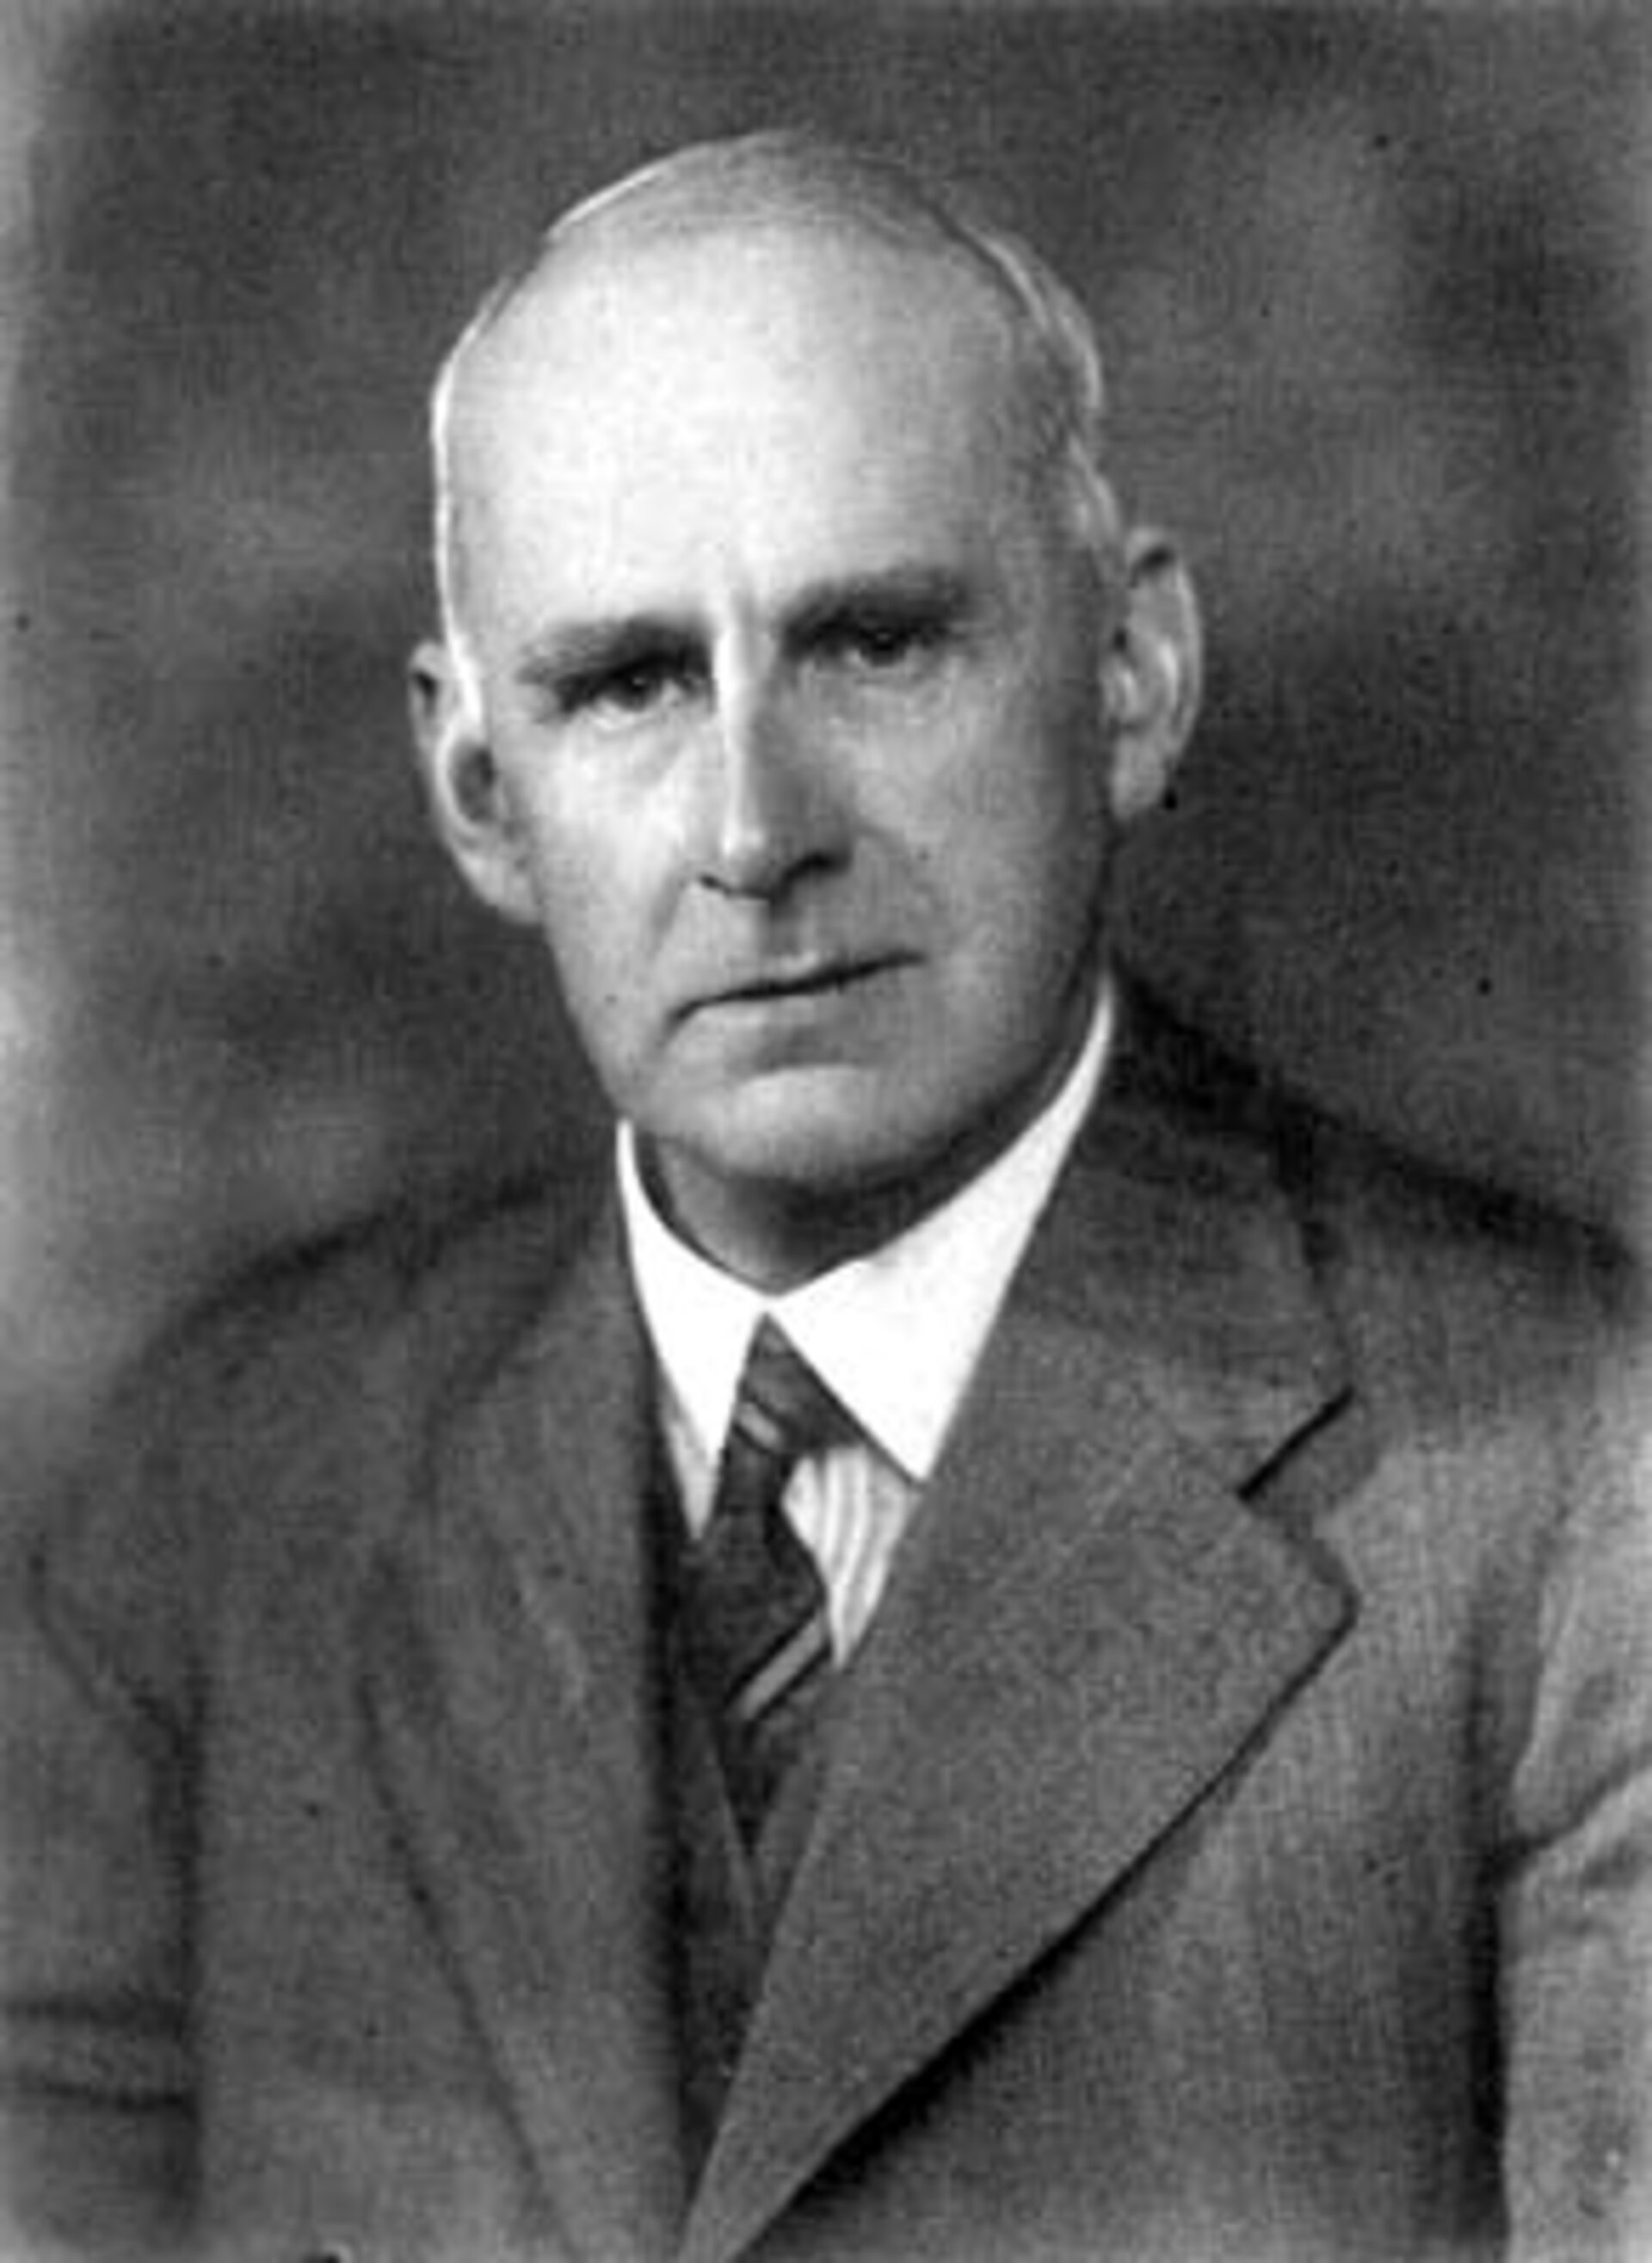
\includegraphics[height=6cm]{Arthur_Stanley_Eddington_1882_-_1944_pillars.jpg}
    \scalebox{.4}{https://www.esa.int/var/esa/storage/images/esa\_multimedia/images/2003/07/arthur\_stanley\_eddington\_1882\_-\_1944/9583215-3-eng-GB/Arthur\_Stanley\_Eddington\_1882\_-\_1944\_pillars.jpg}
    \scalebox{.4}{https://www.bbvaopenmind.com/wp-content/uploads/2019/05/Eddington-3-1-1.jpg}
    \end{column}
    \begin{column}{8cm}

    \begin{varblock}
    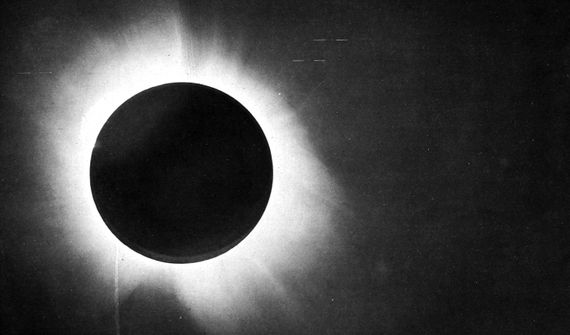
\includegraphics[height=4cm]{Eddington-3-1-1.jpg}
    
    \vspace{1cm}
    \large\texit{"They propagate at the speed of thought"}\\
    \large"-Eddington 1922"
   % \Huge\[h=\frac{2G}{c{^4}}\frac{1}{r}\frac{\delta{^2}Q}{\delta t{^2}}\]
    \end{varblock}
    \end{column}
    \end{columns}
     
\end{frame}
%---------------------------------------------

\begin{frame}{Feliz Pirani and Richard Feynman}
    %\centering
    \begin{columns}[t]
    \begin{column}{4cm}
    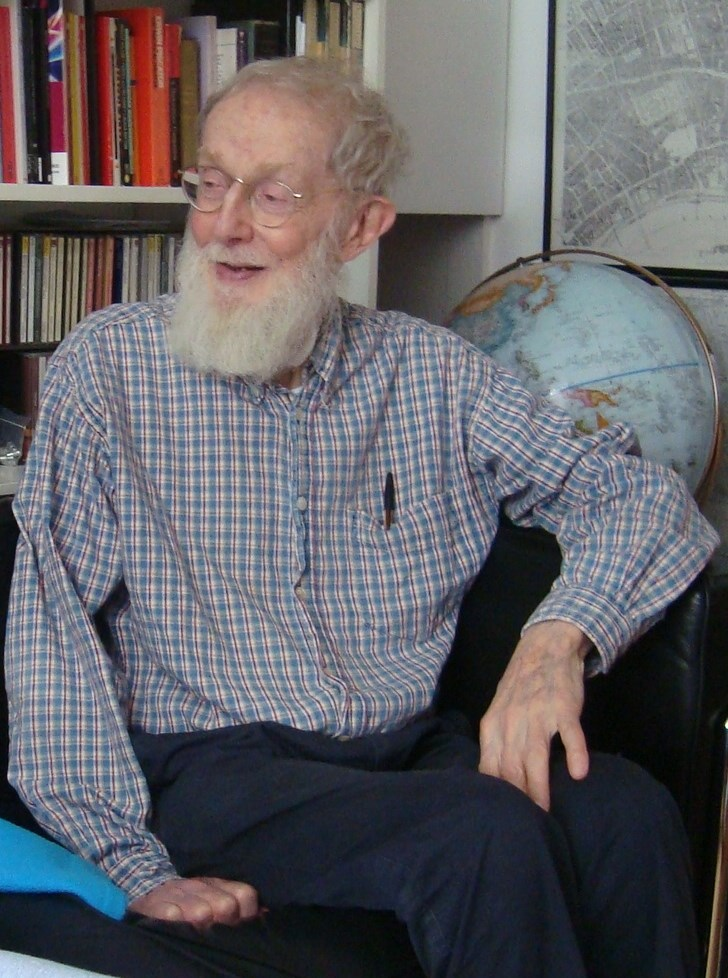
\includegraphics[height=6cm]{pirani.jpg}
    \scalebox{.4}{https://felix-pirani.muchloved.com/}
    \end{column}

    \begin{column}{4cm}
    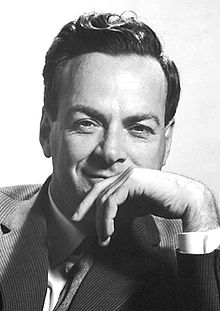
\includegraphics[height=6cm]{Feynman.jpg}
    \scalebox{.4}{https://upload.wikimedia.org/wikipedia/en/thumb/4/42/Richard\_Feynman\_Nobel.jpg/220px-Richard\_Feynman\_Nobel.jpg}
    \end{column}
  
    \end{columns}
     
\end{frame}
%---------------------------------------------
\fi
\begin{frame}{First Measurement of Gravitational Waves}
    %\centering
    \begin{columns}[t]
    \begin{column}{6cm}
    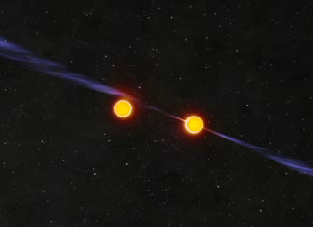
\includegraphics[height=5cm]{BinaryPulsar.png}
    \scalebox{.4}{https://astrobites.org/wp-content/uploads/2018/02/BinaryPulsar.png}
    \end{column}

    \begin{column}{5cm}
    %\vspace{0.5cm}
    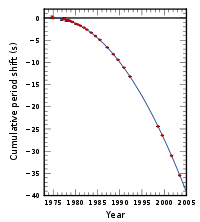
\includegraphics[height=5.5cm]{htbp.png}
    \scalebox{.4}{\(\;\;\;\;\;\;\;\;\;\)https://en.wikipedia.org/wiki/Hulse\%E2\%80\%93Taylor\_binary}
    
    \end{column}
  
    \end{columns}
\end{frame}
%---------------------------------------------

\begin{frame}{Gravitational Waves}
   \centering
    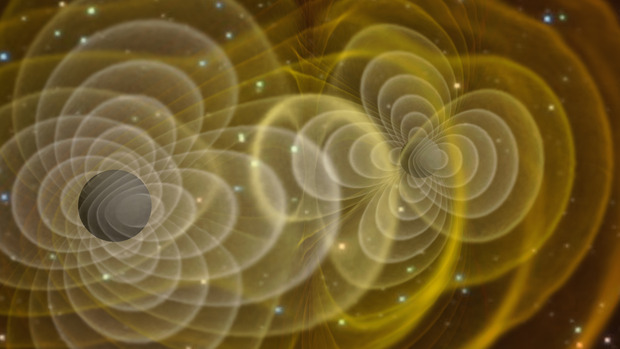
\includegraphics[height=7cm]{gw.jpg}\\
     \scalebox{.4}{ https://www.ligo.caltech.edu/page/what-are-gw}

\end{frame}
%------------------------------------------------
\begin{frame}{Laser Intereferometry}
   \centering
    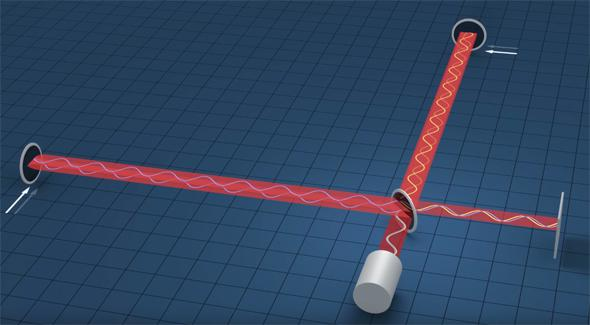
\includegraphics[height=7cm]{li2.jpg}\\
     \scalebox{.4}{https://slate.com/technology/2017/01/derek-muller-investigates-ligo.html}

\end{frame}
%---------------------------------------------
\begin{frame}{Laser Interferometer Gravitational-Wave Observatory (LIGO)}
    \centering
    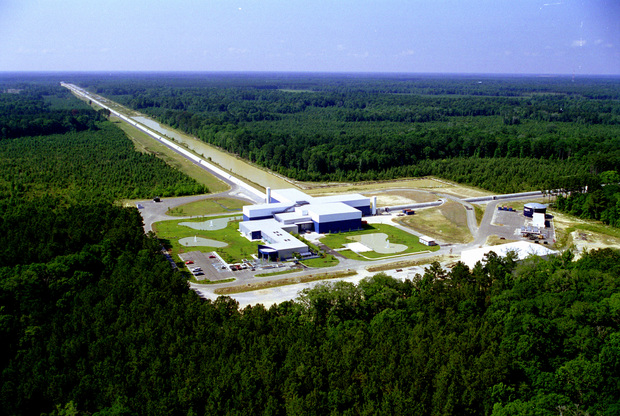
\includegraphics[height=6.3cm]{ligo.jpg}\\
     \scalebox{.4}{https://www.google.com/search?q=nasa+lisa&tbm=isch#imgrc=YPfHoKiLKPAmLM}
\end{frame}
%------------------------------------------------
\begin{frame}{Laser Interferometer Space Antenna (LISA)}
    \centering
    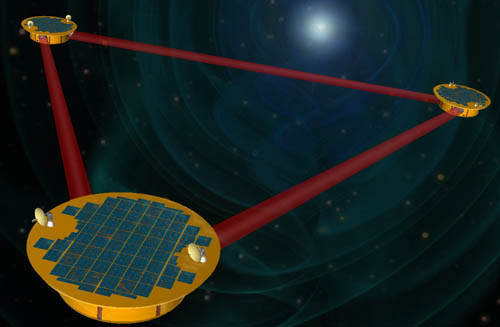
\includegraphics[height=7cm]{LISA.jpg}\\
    \scalebox{.4}{https://lisa.nasa.gov/archive2011/}
\end{frame}
%------------------------------------------------
\begin{frame}{Laser Interferometer Space Antenna (LISA)}
    \centering
    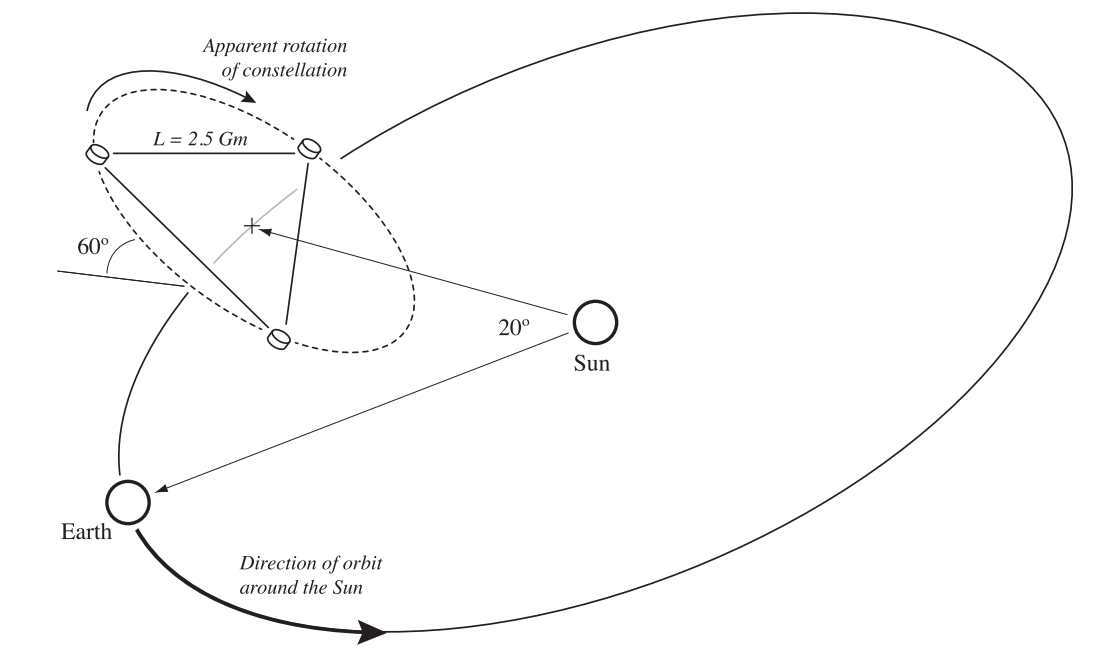
\includegraphics[height=7cm]{figure 1.png}\\
    \scalebox{.4}{https://arxiv.org/pdf/1912.07715.pdf}
 \end{frame}
%------------------------------------------------
\begin{frame}{LISA Pathfinder (LPF)}
    \centering
    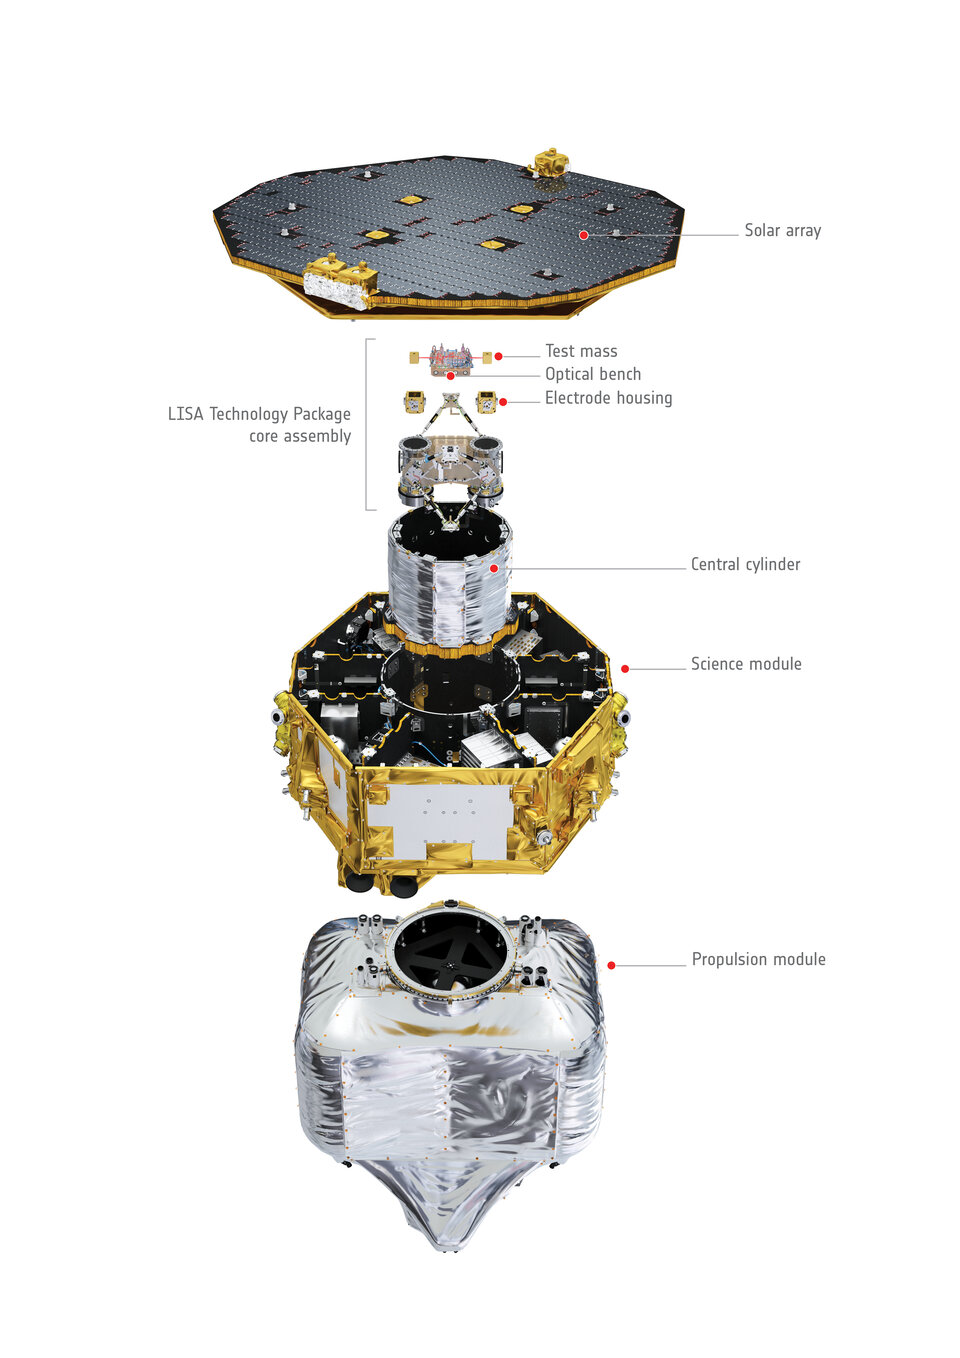
\includegraphics[height=7cm]{LPF.jpg}\\
    \scalebox{.4}{https://www.esa.int/Enabling\_Support/Operations/LISA\_Pathfinder}
\end{frame}
%------------------------------------------------
\begin{frame}{LISA Pathfinder (LPF)}
    \centering
    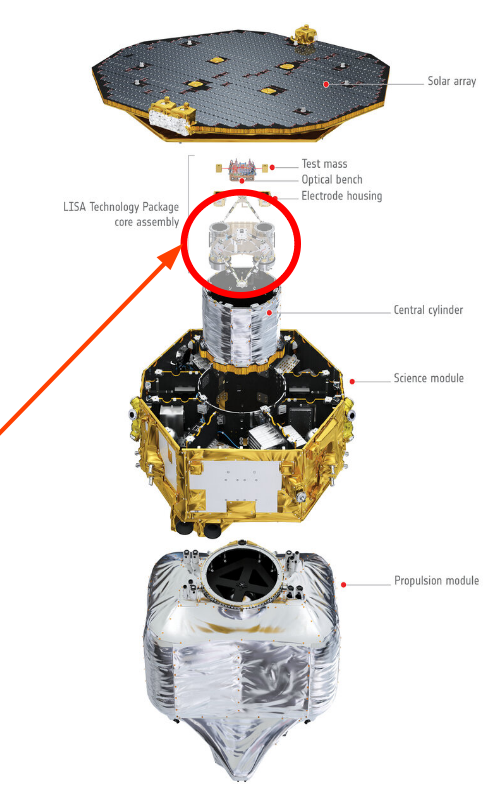
\includegraphics[height=7cm]{LISA_Pathfinder_exploded_view_article}\\
    \scalebox{.4}{https://www.esa.int/Enabling\_Support/Operations/LISA\_Pathfinder}
\end{frame}
%------------------------------------------------
\begin{frame}{Laser Interferometer Space Antenna (LISA)}
    \centering
    %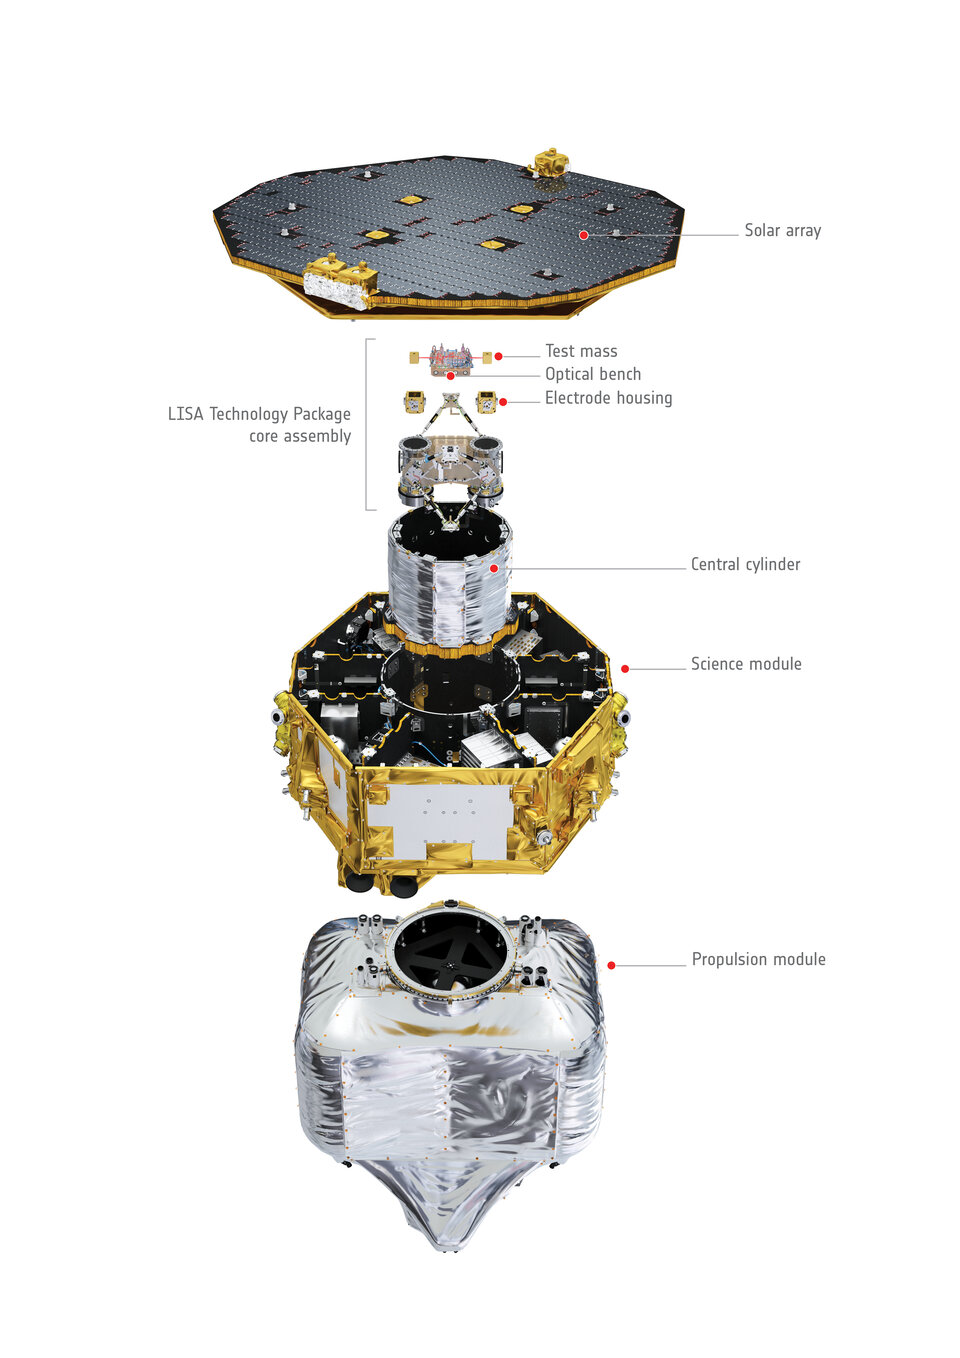
\includegraphics[height=7cm]{LPF.jpg}\\
    %\scalebox{.4}{https://www.esa.int/Enabling\_Support/Operations/LISA\_Pathfinder}
    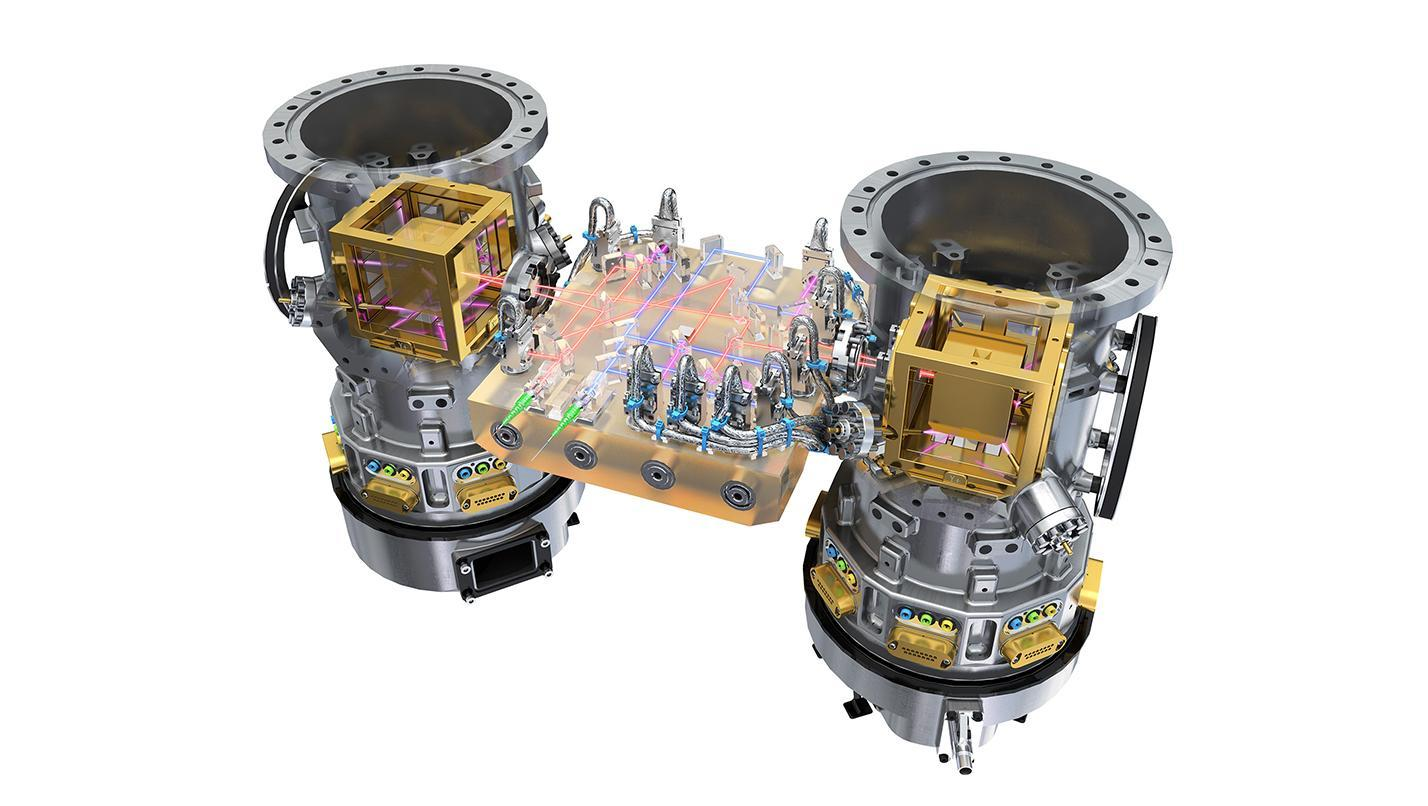
\includegraphics[height=7cm]{lisatech.jpg}\\
    \scalebox{.4}{https://www.dlr.de/content/en/articles/news/2015/20151203\_in-the-footprints-of-albert-einstein-successful-launch-of-lisa-pathfinder\_15996.html}
\end{frame}
%------------------------------------------------
\begin{frame}{Solar Wind}
    \centering
    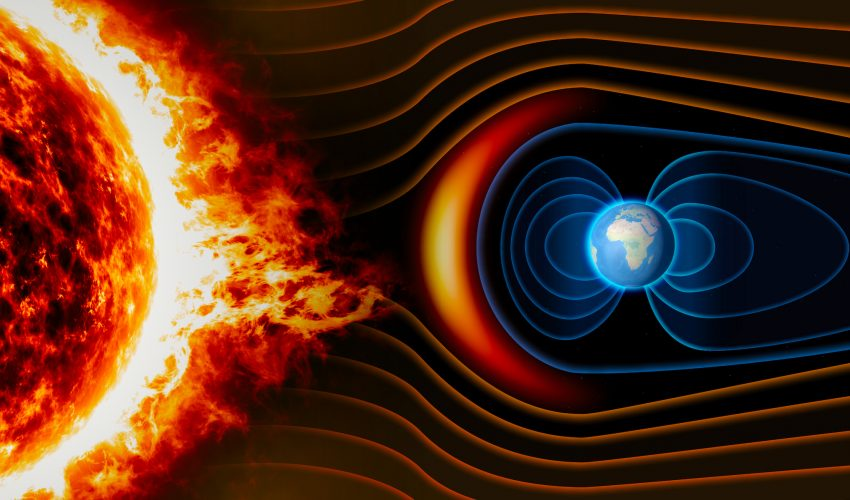
\includegraphics[height=7cm]{solarwind.jpg}\\
    \scalebox{.4}{https://www.earth.com/news/solar-wind-collides-magnetic-field/}
\end{frame}
%------------------------------------------------
\begin{frame}{Advanced Composition Explorer (ACE)}
\centering
    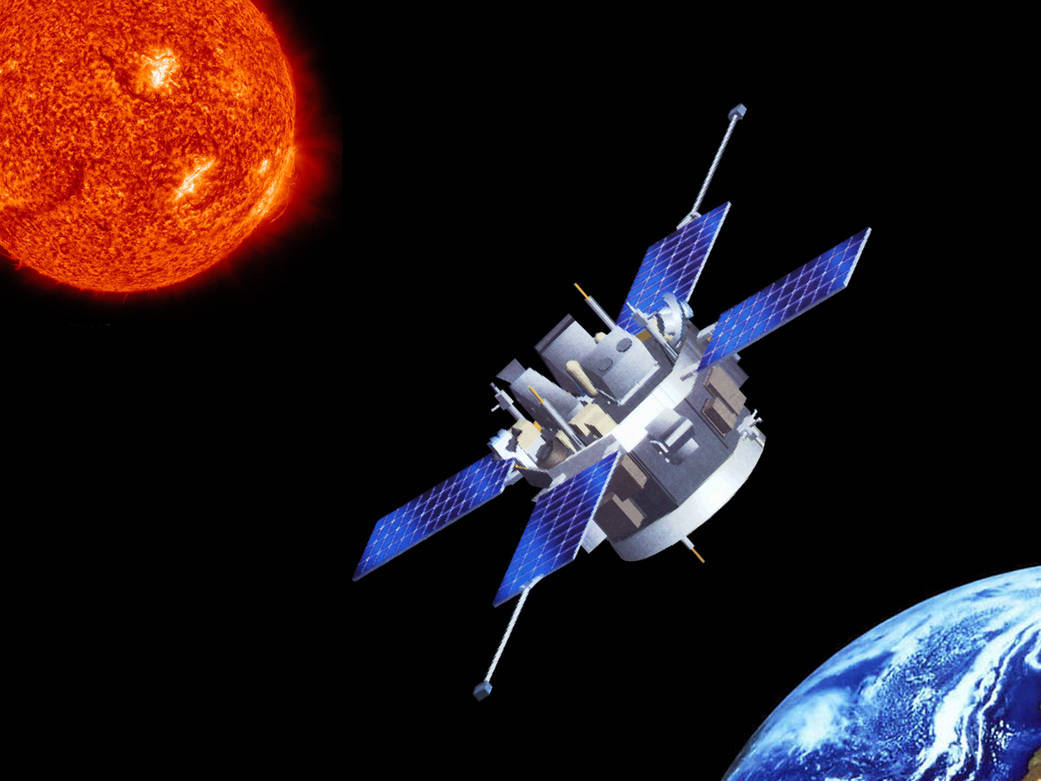
\includegraphics[height=7cm]{ACE.jpg}\\
    \scalebox{.4}{https://solarsystem.nasa.gov/missions/ace/in-depth/}
\end{frame}
%------------------------------------------------
\begin{frame}{Lagrange Points}
   \centering
    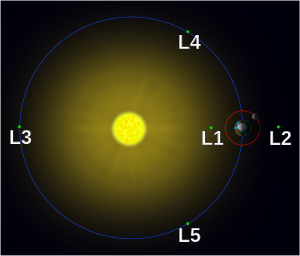
\includegraphics[height=7cm]{lagrange.png}\\
    \scalebox{.4}{ https://en.wikipedia.org/wiki/Lagrange_point}
\end{frame}
%------------------------------------------------
\begin{frame}{Methods}
\centering
    
\includegraphics[height=3.5cm, width=14.5cm]{fig1solWmam.jpg}
\end{frame}
%------------------------------------------------
\begin{frame}{Gap Filling}
    \begin{table}[htbp]

    \begin{center}
    \renewcommand{\arraystretch}{1.5}
    \begin{tabular}{|c|c|c|}
    \hline
    %\textbf{Table}&\multicolumn{3}{|c|}{\textbf{Table Column Head}} \\
    Type & Length & Fill Method\\
    %\textbf{Head} & \textbf{\textit{Table column subhead}}& \textbf{\textit{Subhead}}& \textbf{\textit{Subhead}} \\
    \hline
    A & 1 & Linear Interpolation\\
    \hline
    B & 2-24 & Gaussian Noise with Linear Interpolation\\
    \hline
    C & $\geq$25 & Hann Window\\
    \hline
    %copy& More table copy$^{\mathrm{a}}$& &  \\
    
    %\multicolumn{4}{l}
    %\multicolumn{4}{l}{$^{\mathrm{a}}$P values were computed by the Mann-Whitney-U test.}
    \end{tabular}
    \label{tab1}
    \end{center}
    \end{table}\\
Gaussian Noise: 
\begin{equation}\label{eq:Gaussian Window Equations}
\sigma=\frac{l-(i-1)}{l+1}\sigma_{1}+\frac{i}{l+1}\sigma_{2}
\end{equation}
Hann Window:
where \textit{N}=51 and 0$<$\textit{n}$<$\textit{N}-1
\begin{equation}\label{eq:Hanning Window}
\omega(n)=0.5\biggr[1-\cos{\biggl(\frac{2\pi n}{N-1}\biggl)}\biggr]
\end{equation}\\
\end{frame}
%------------------------------------------------
\begin{frame}{Gaussian and Hann Window}
\begin{columns}[t]
    \begin{column}{6cm}
    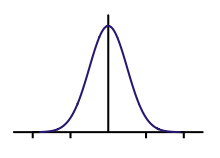
\includegraphics[height=7cm, width=7cm]{gaussian.png}
    \scalebox{.4}{https://en.wikipedia.org/wiki/Gaussian\_filter}
    \end{column}
    \begin{column}{7cm}
    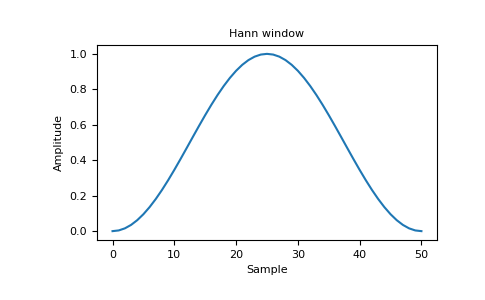
\includegraphics[height=7cm, width=7.5cm]{hann.png}
    \scalebox{.4}{ https://numpy.org/doc/stable/reference/generated/numpy.hanning.html}
    \end{column}
\end{columns}
\end{frame}
%------------------------------------------------
\begin{frame}{Equations}
Number of particles hitting LPF solar array
\begin{equation}\label{eq:Hanning Window}
N=n v Acos(\phi),
\end{equation}
ACE Force:
\begin{equation}\label{eq:Hanning Window}
\begin{split}
F_{x}=(N_{p}m_{p}+N_{\alpha}m_{\alpha})[(1+cos(2\phi))v_{x}+sin(2\phi)v_{z}], \\ F_{y}=0, \\ F_{z}=(N_{p}m_{p}+N_{\alpha}m_{\alpha})[(1+cos(2\phi))v_{z}+sin(2\phi)v_{x}].
\end{split}
\end{equation}
\end{frame}
%------------------------------------------------
\begin{frame}{Time series}
    \centering
    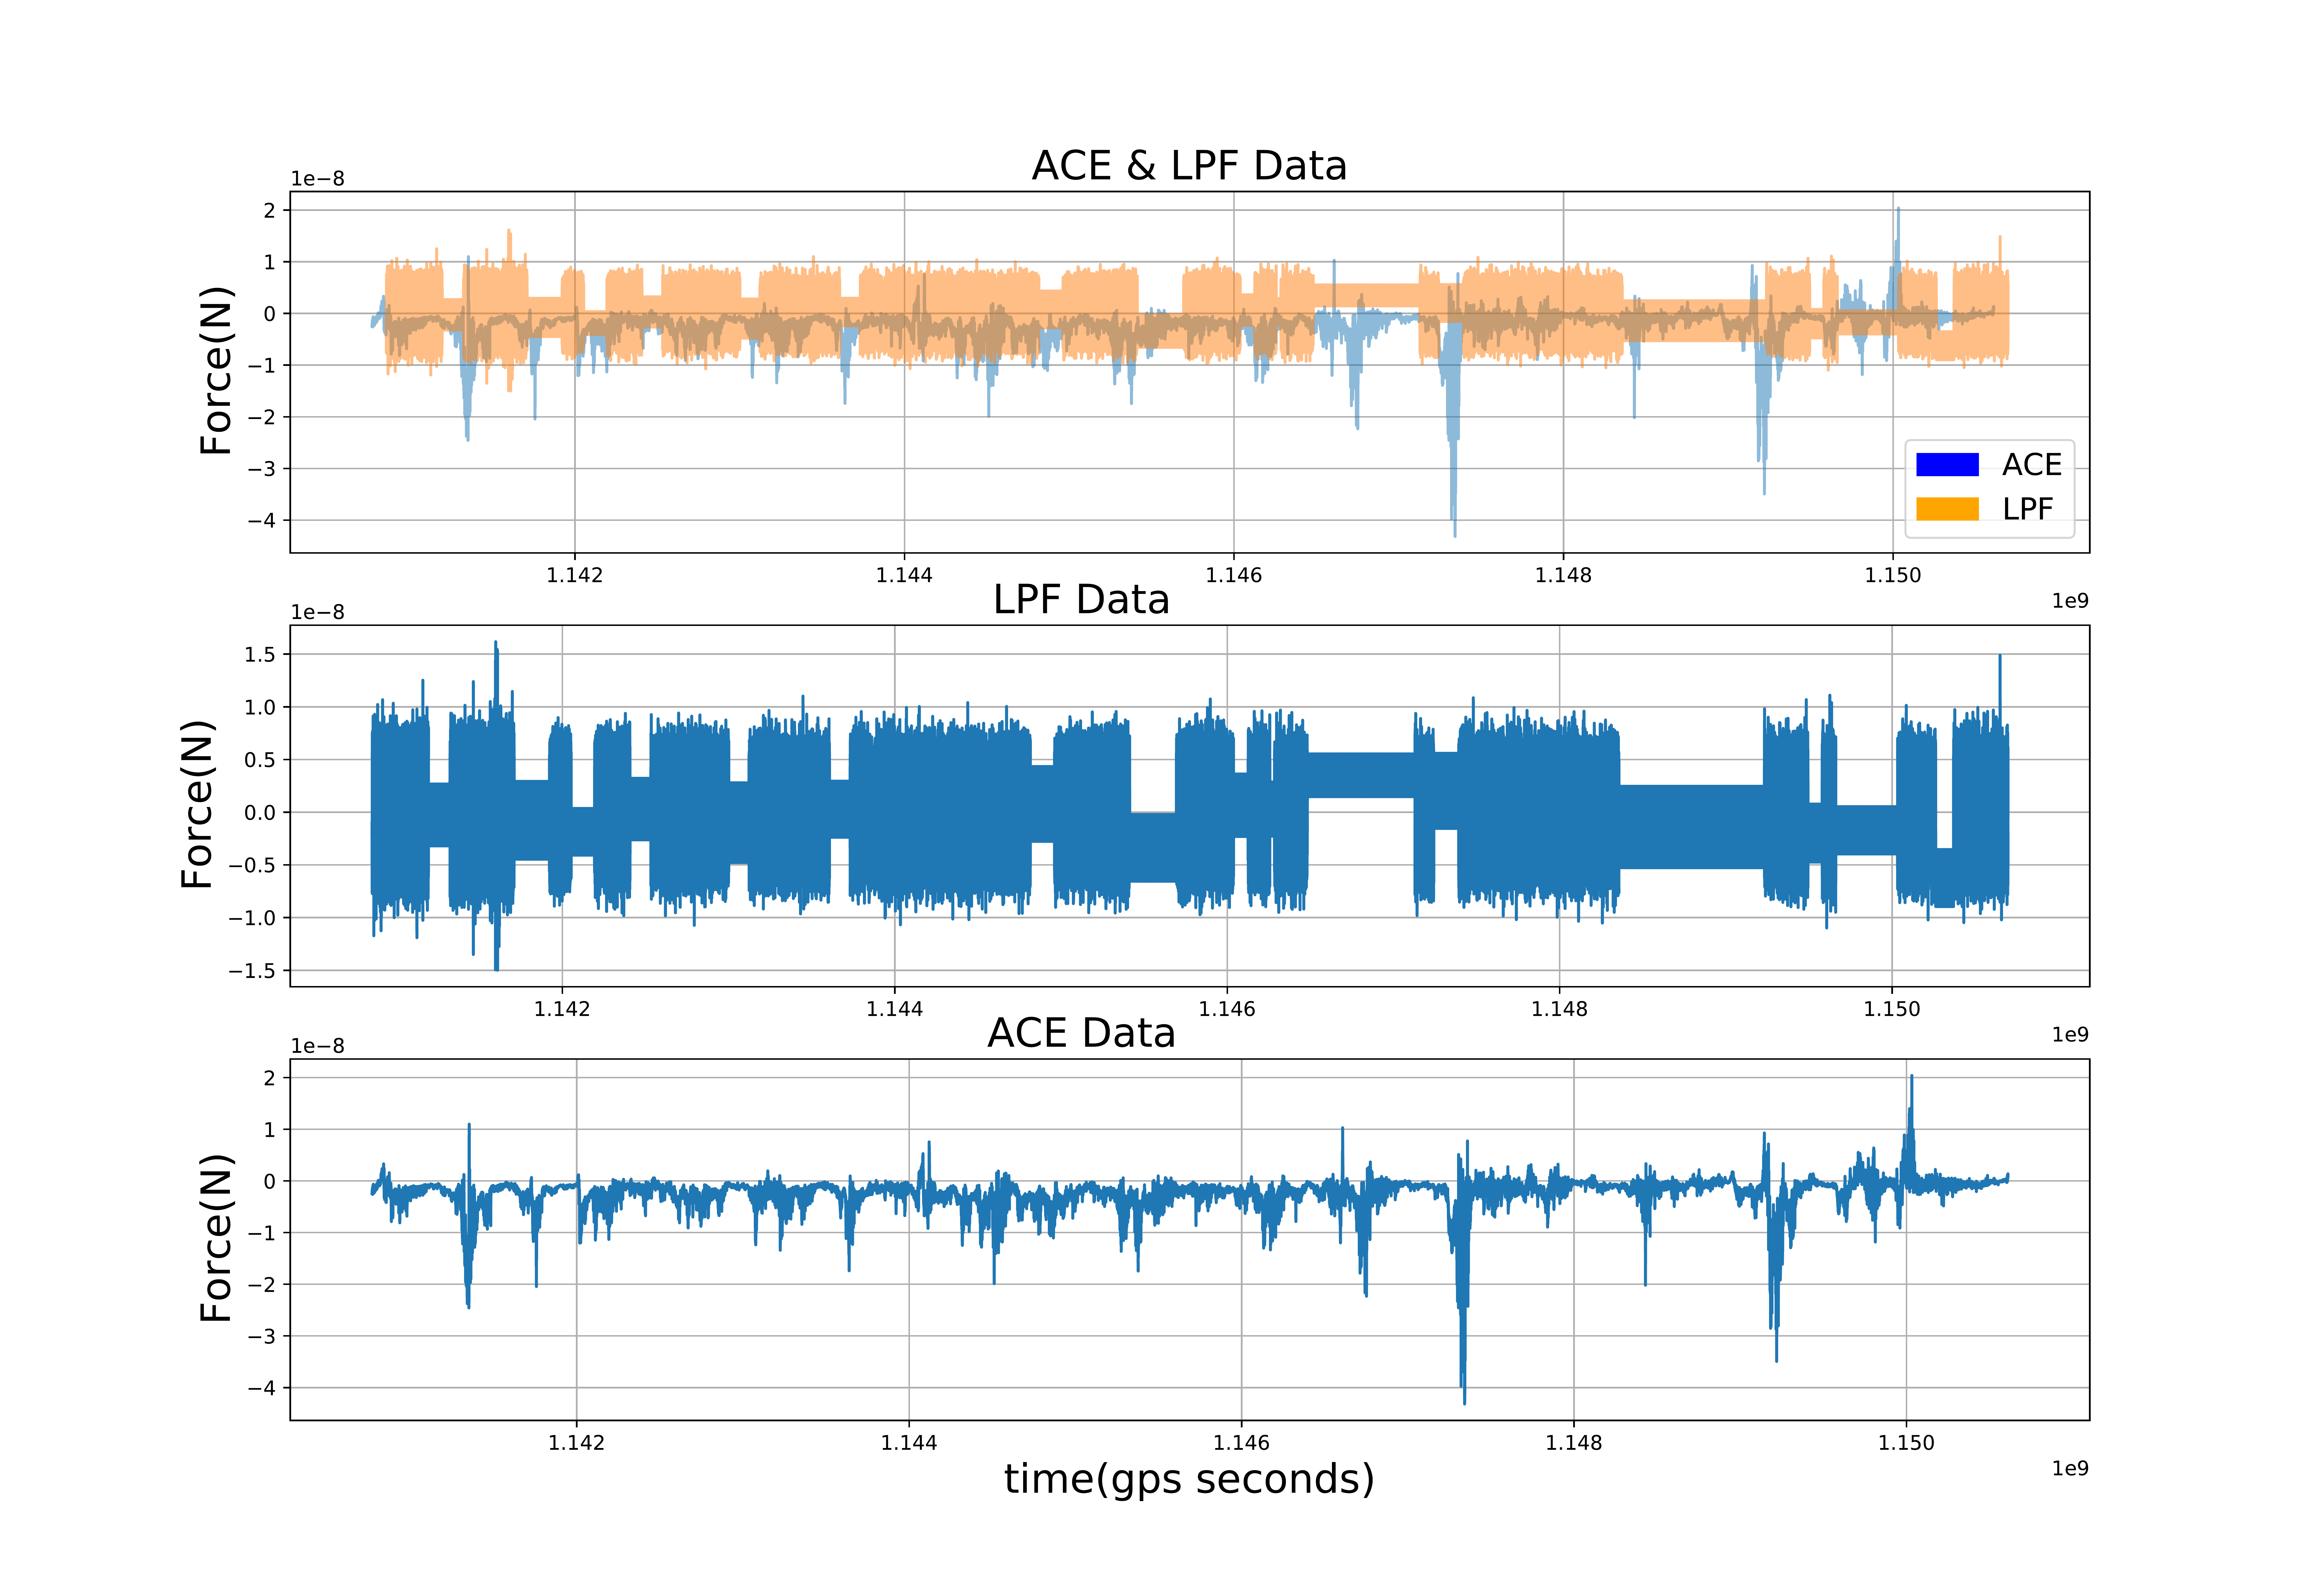
\includegraphics[height=8cm]{TimeDomain_Comparison_ACEvLPF-1.png}
\end{frame}
%------------------------------------------------
\begin{frame}{FFT}
    \centering
    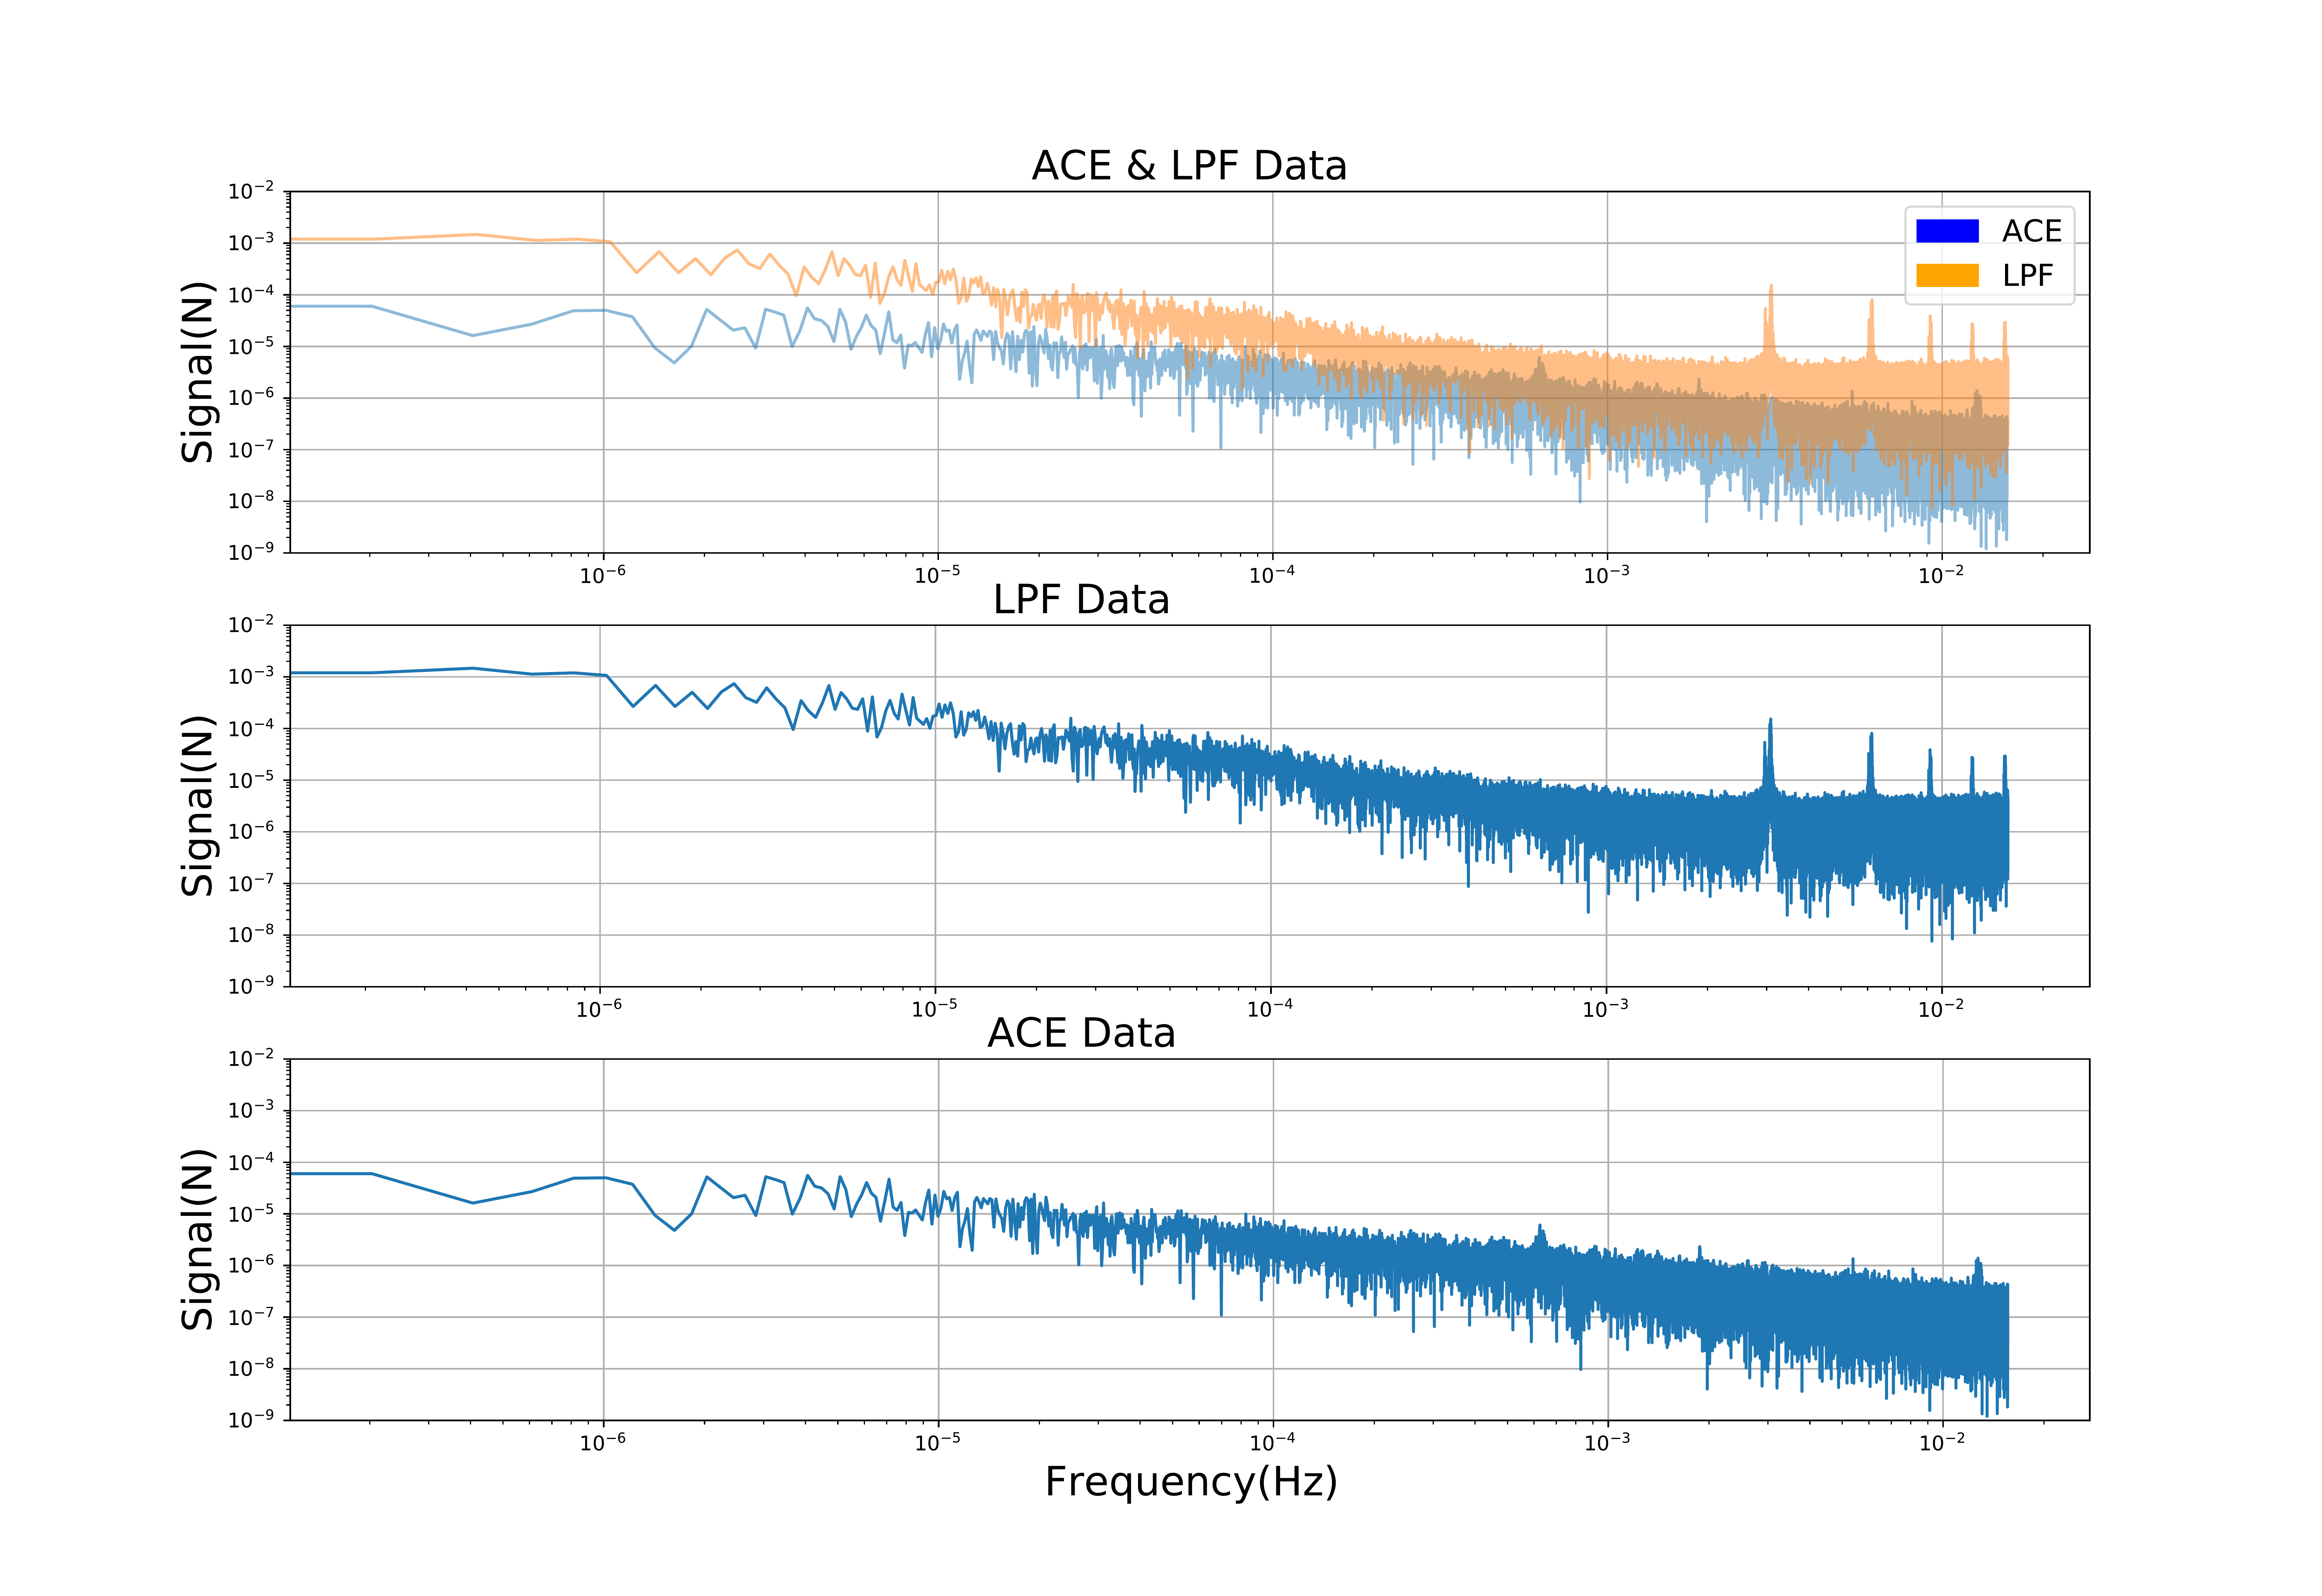
\includegraphics[height=8cm]{ACE_and_LPF_Loglo-1.png}
\end{frame}
\iffalse
%------------------------------------------------
\begin{frame}{Bode Magnitude}
    \centering
    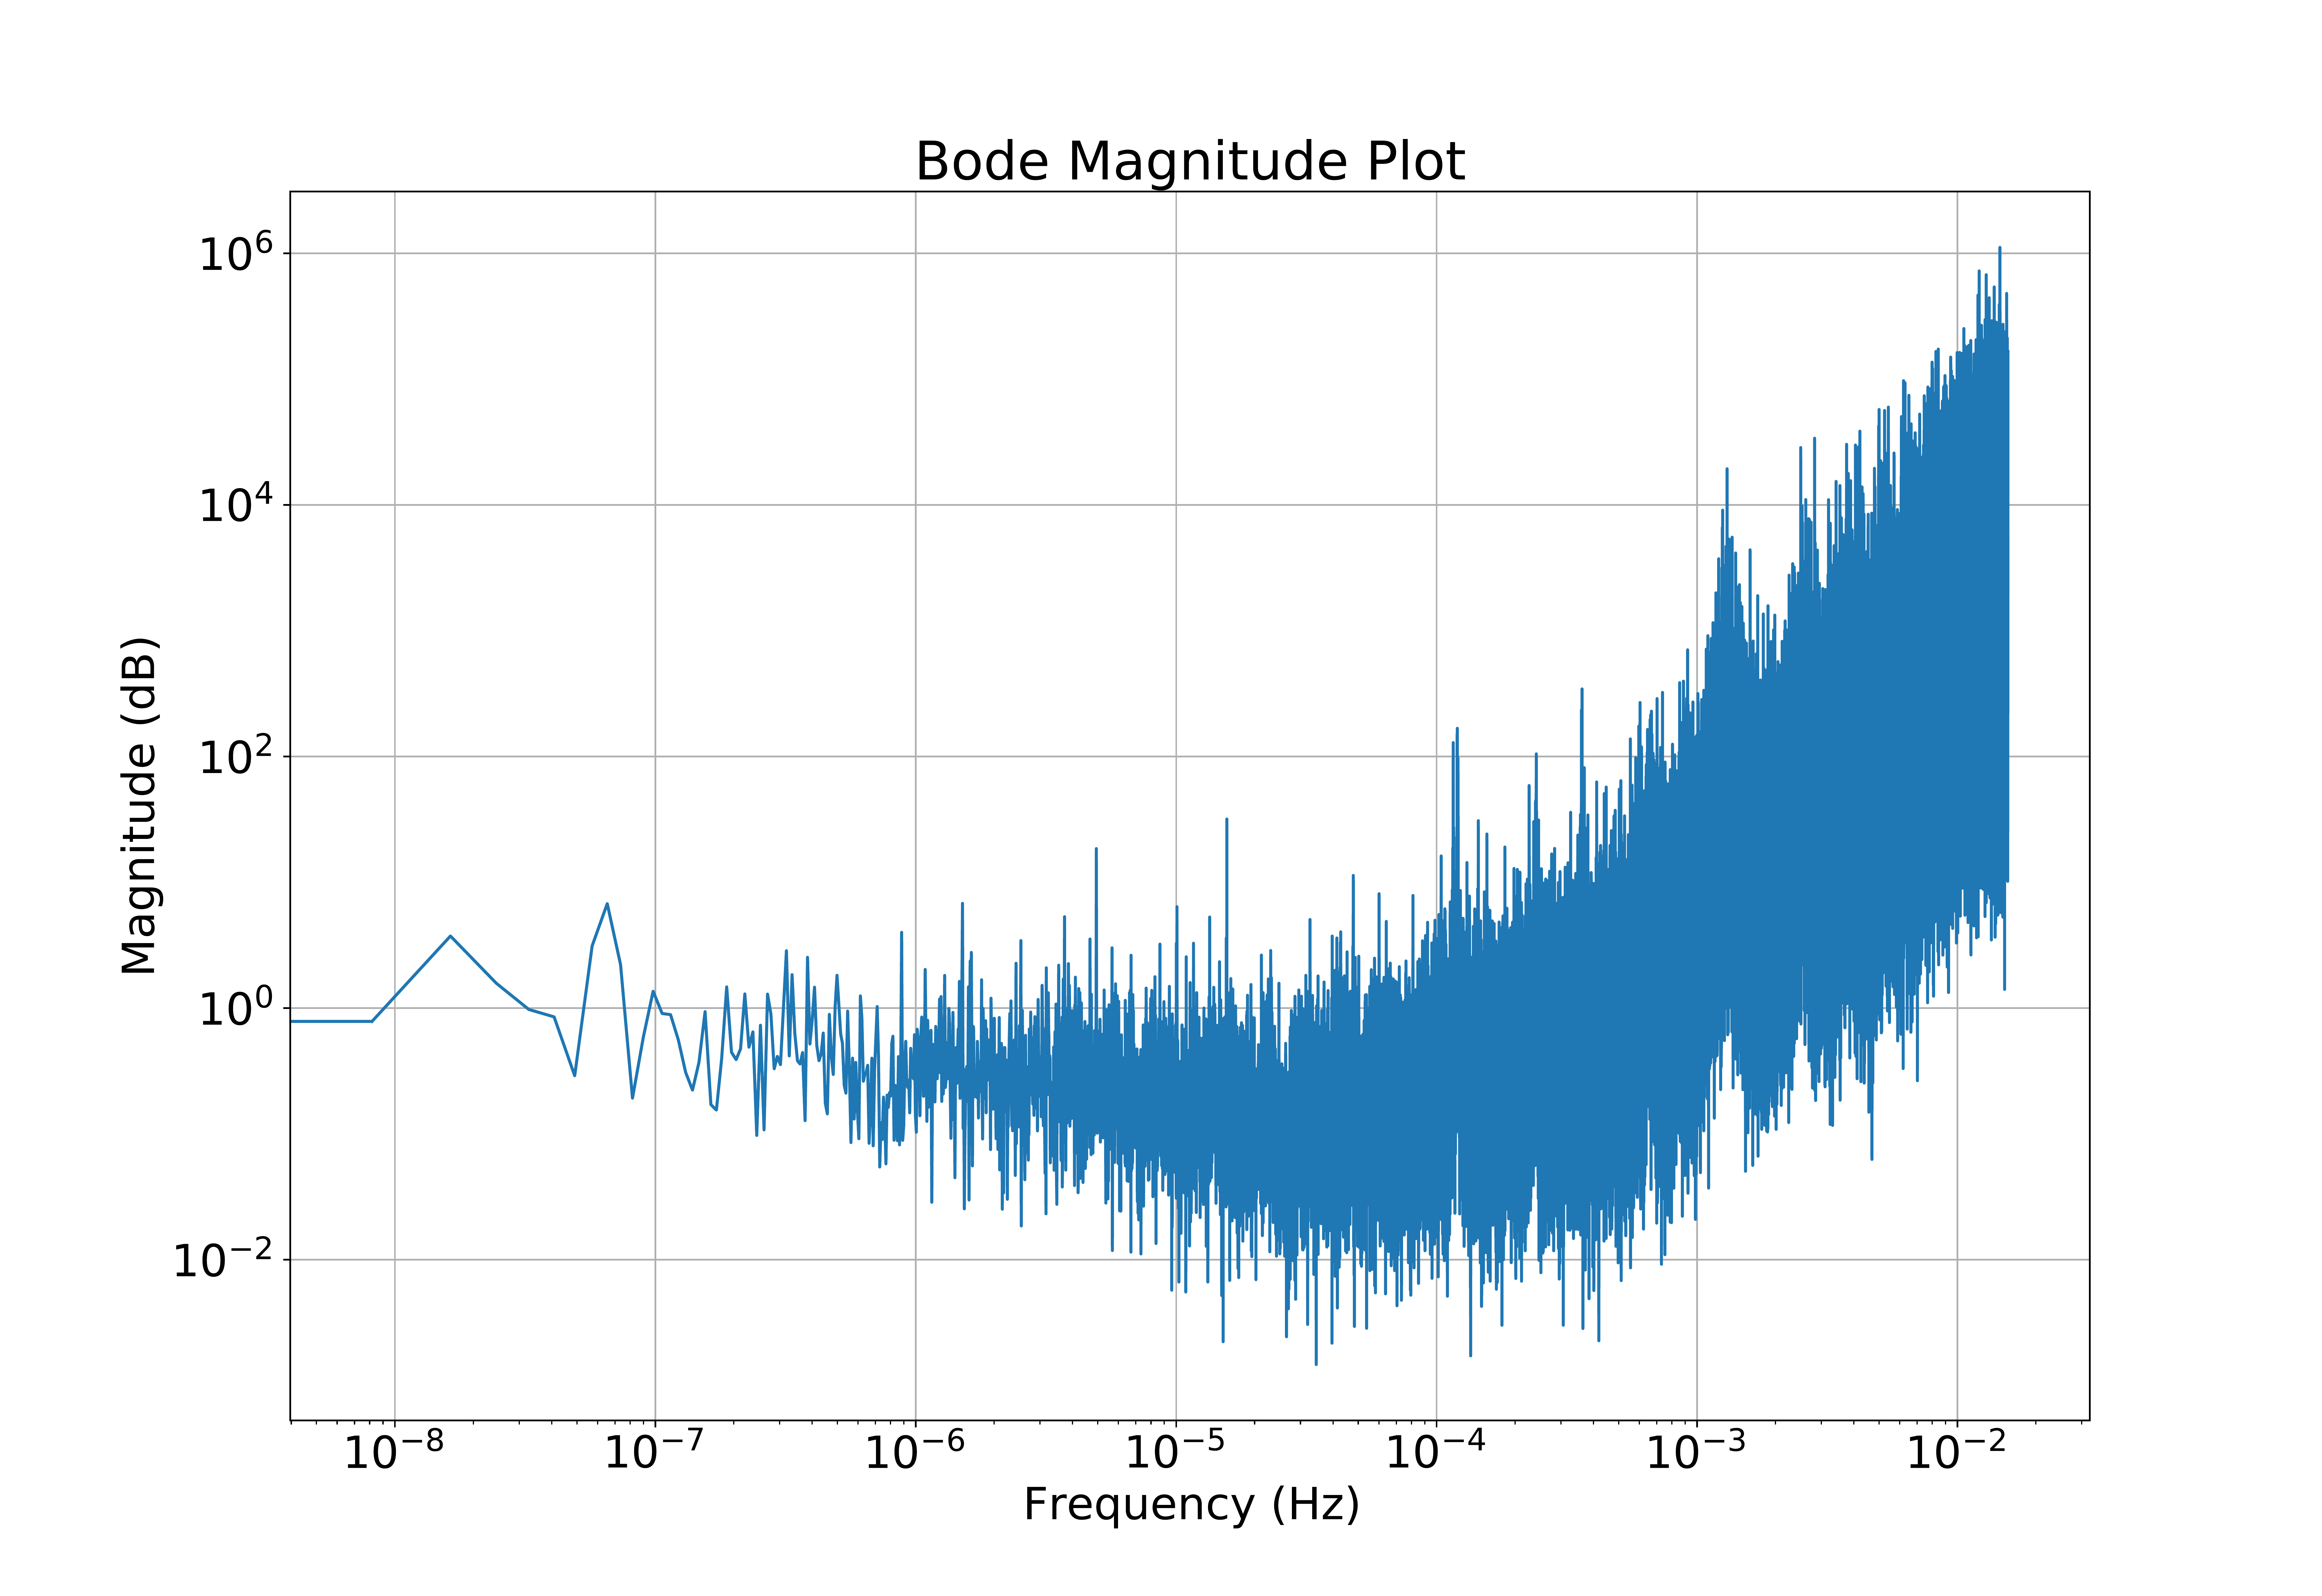
\includegraphics[height=8cm]{Bode_Magnitude_Plot-1.png}
\end{frame}
%------------------------------------------------
\begin{frame}{Bode Phase}
    \centering
    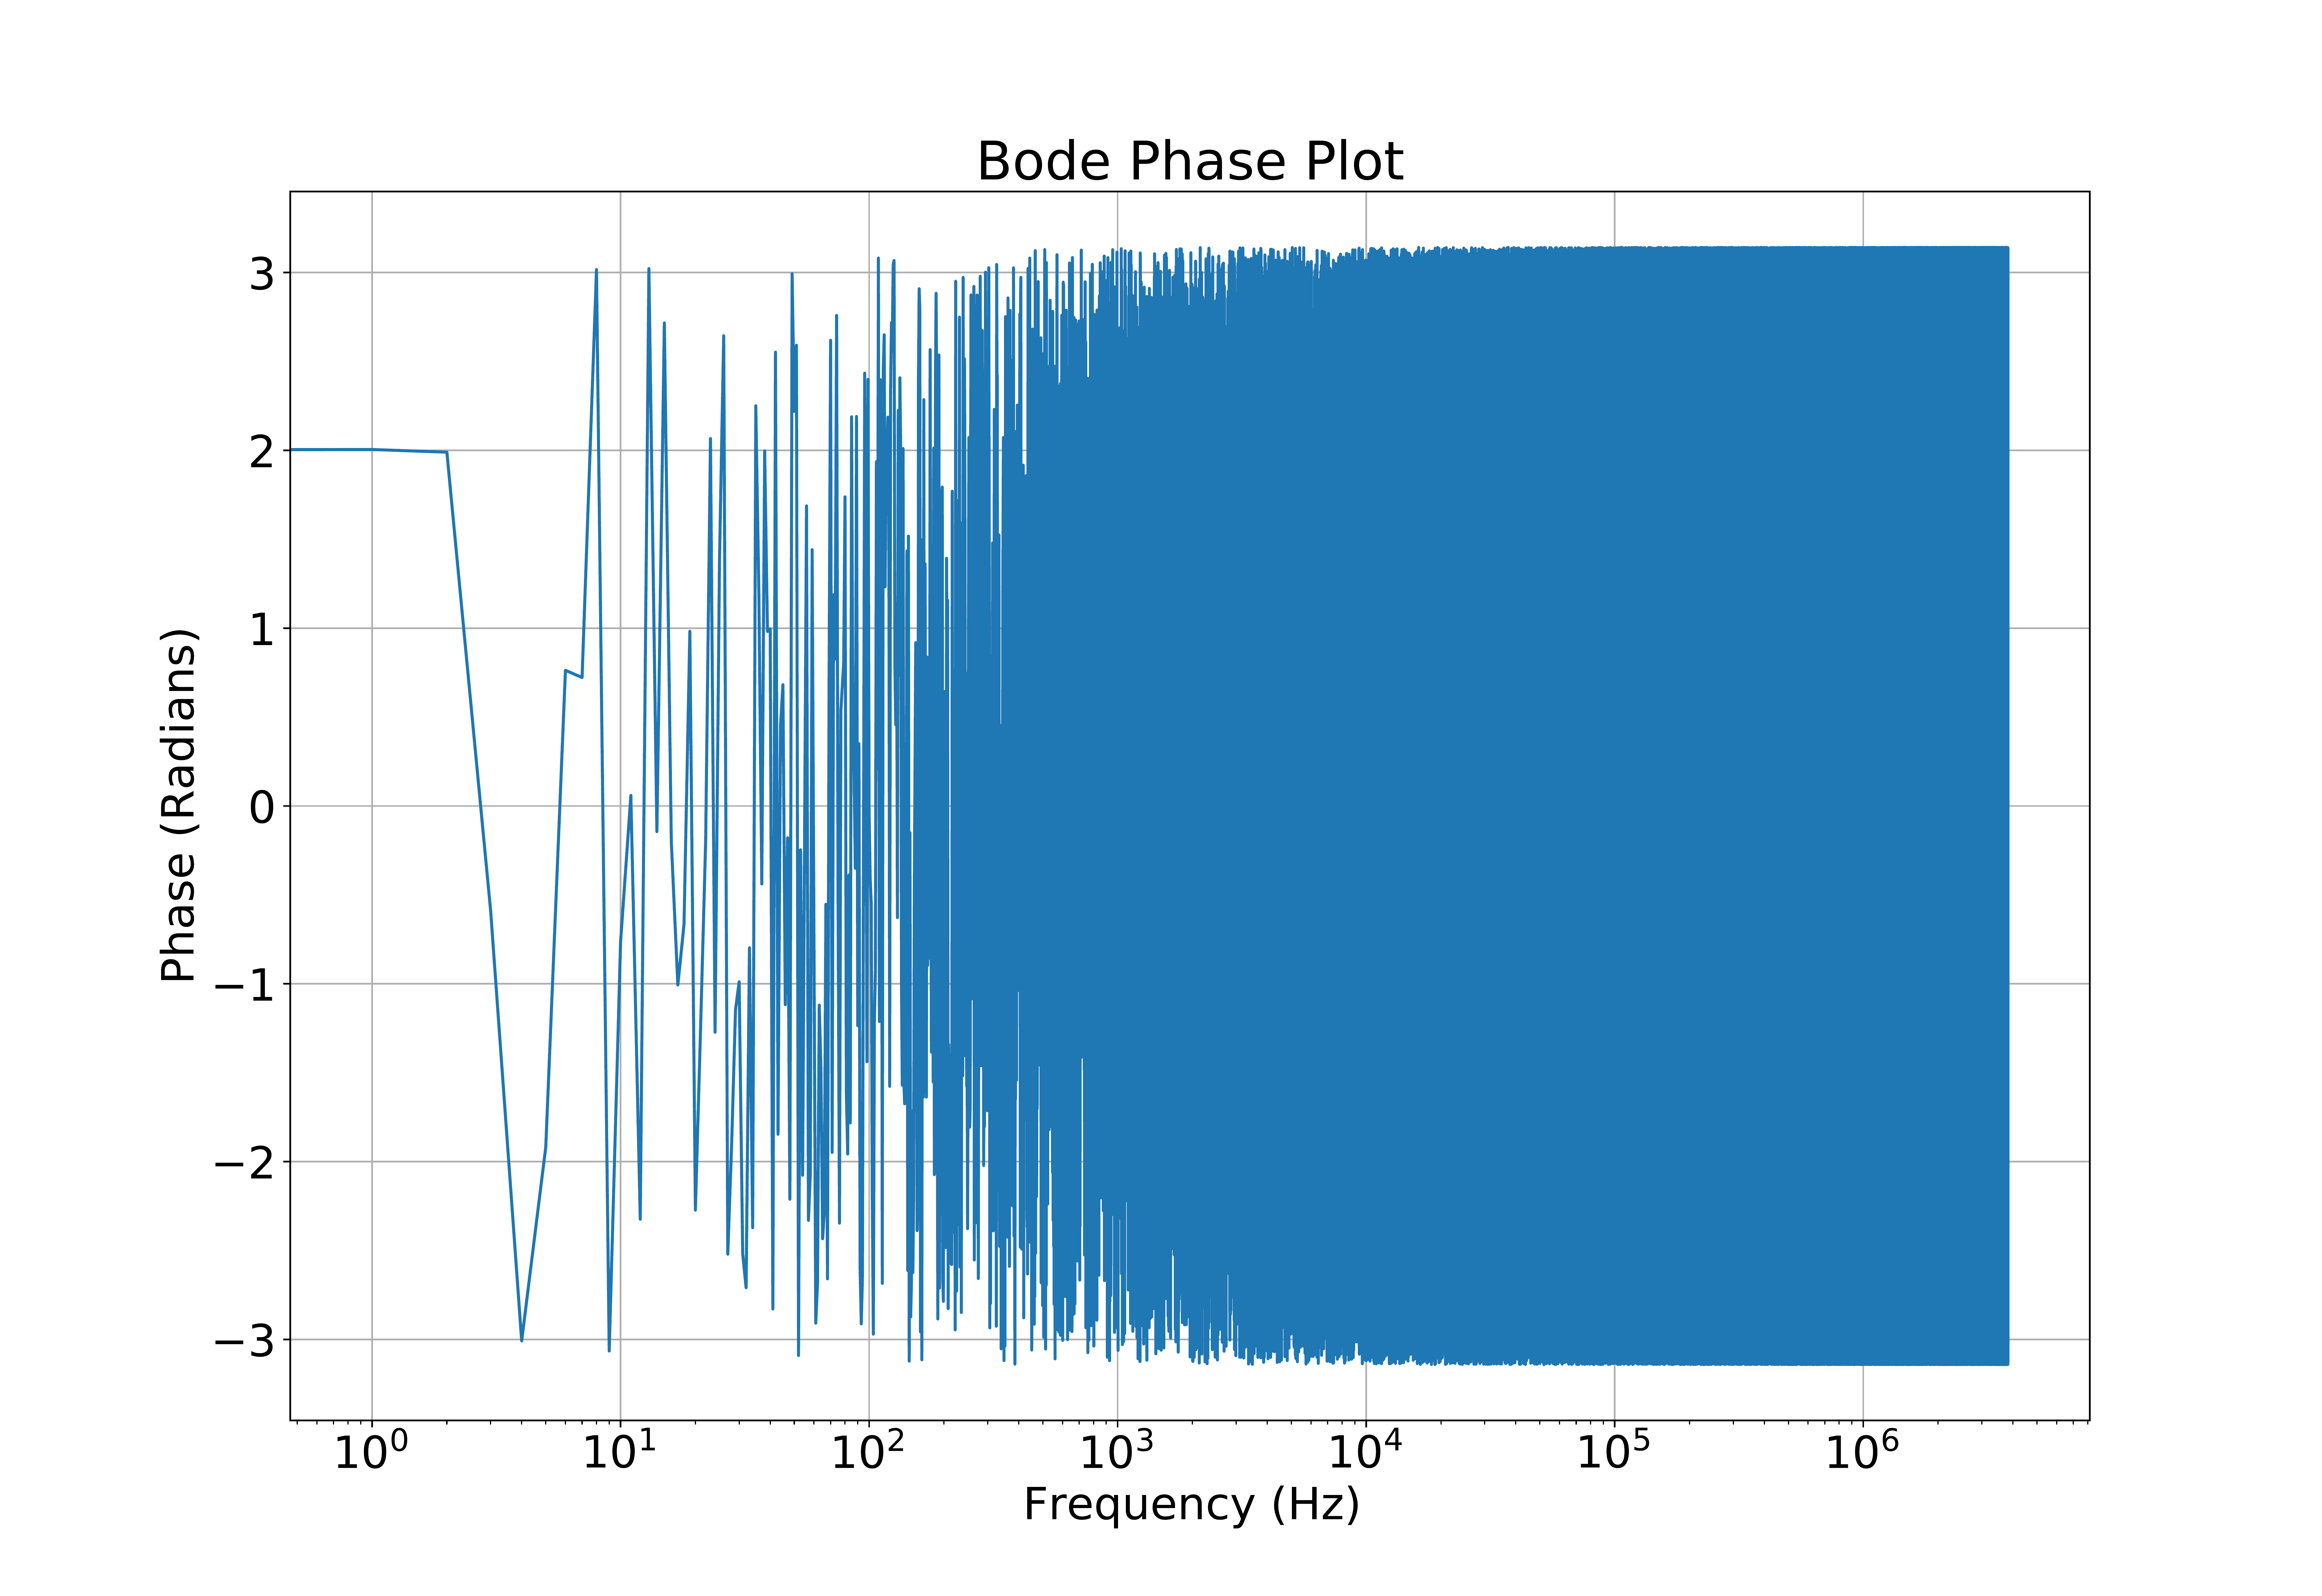
\includegraphics[height=8cm]{Bode_Phase_Plot-1.png}
\end{frame}
\fi
%------------------------------------------------
\begin{frame}{Bode Plot}
    \centering
    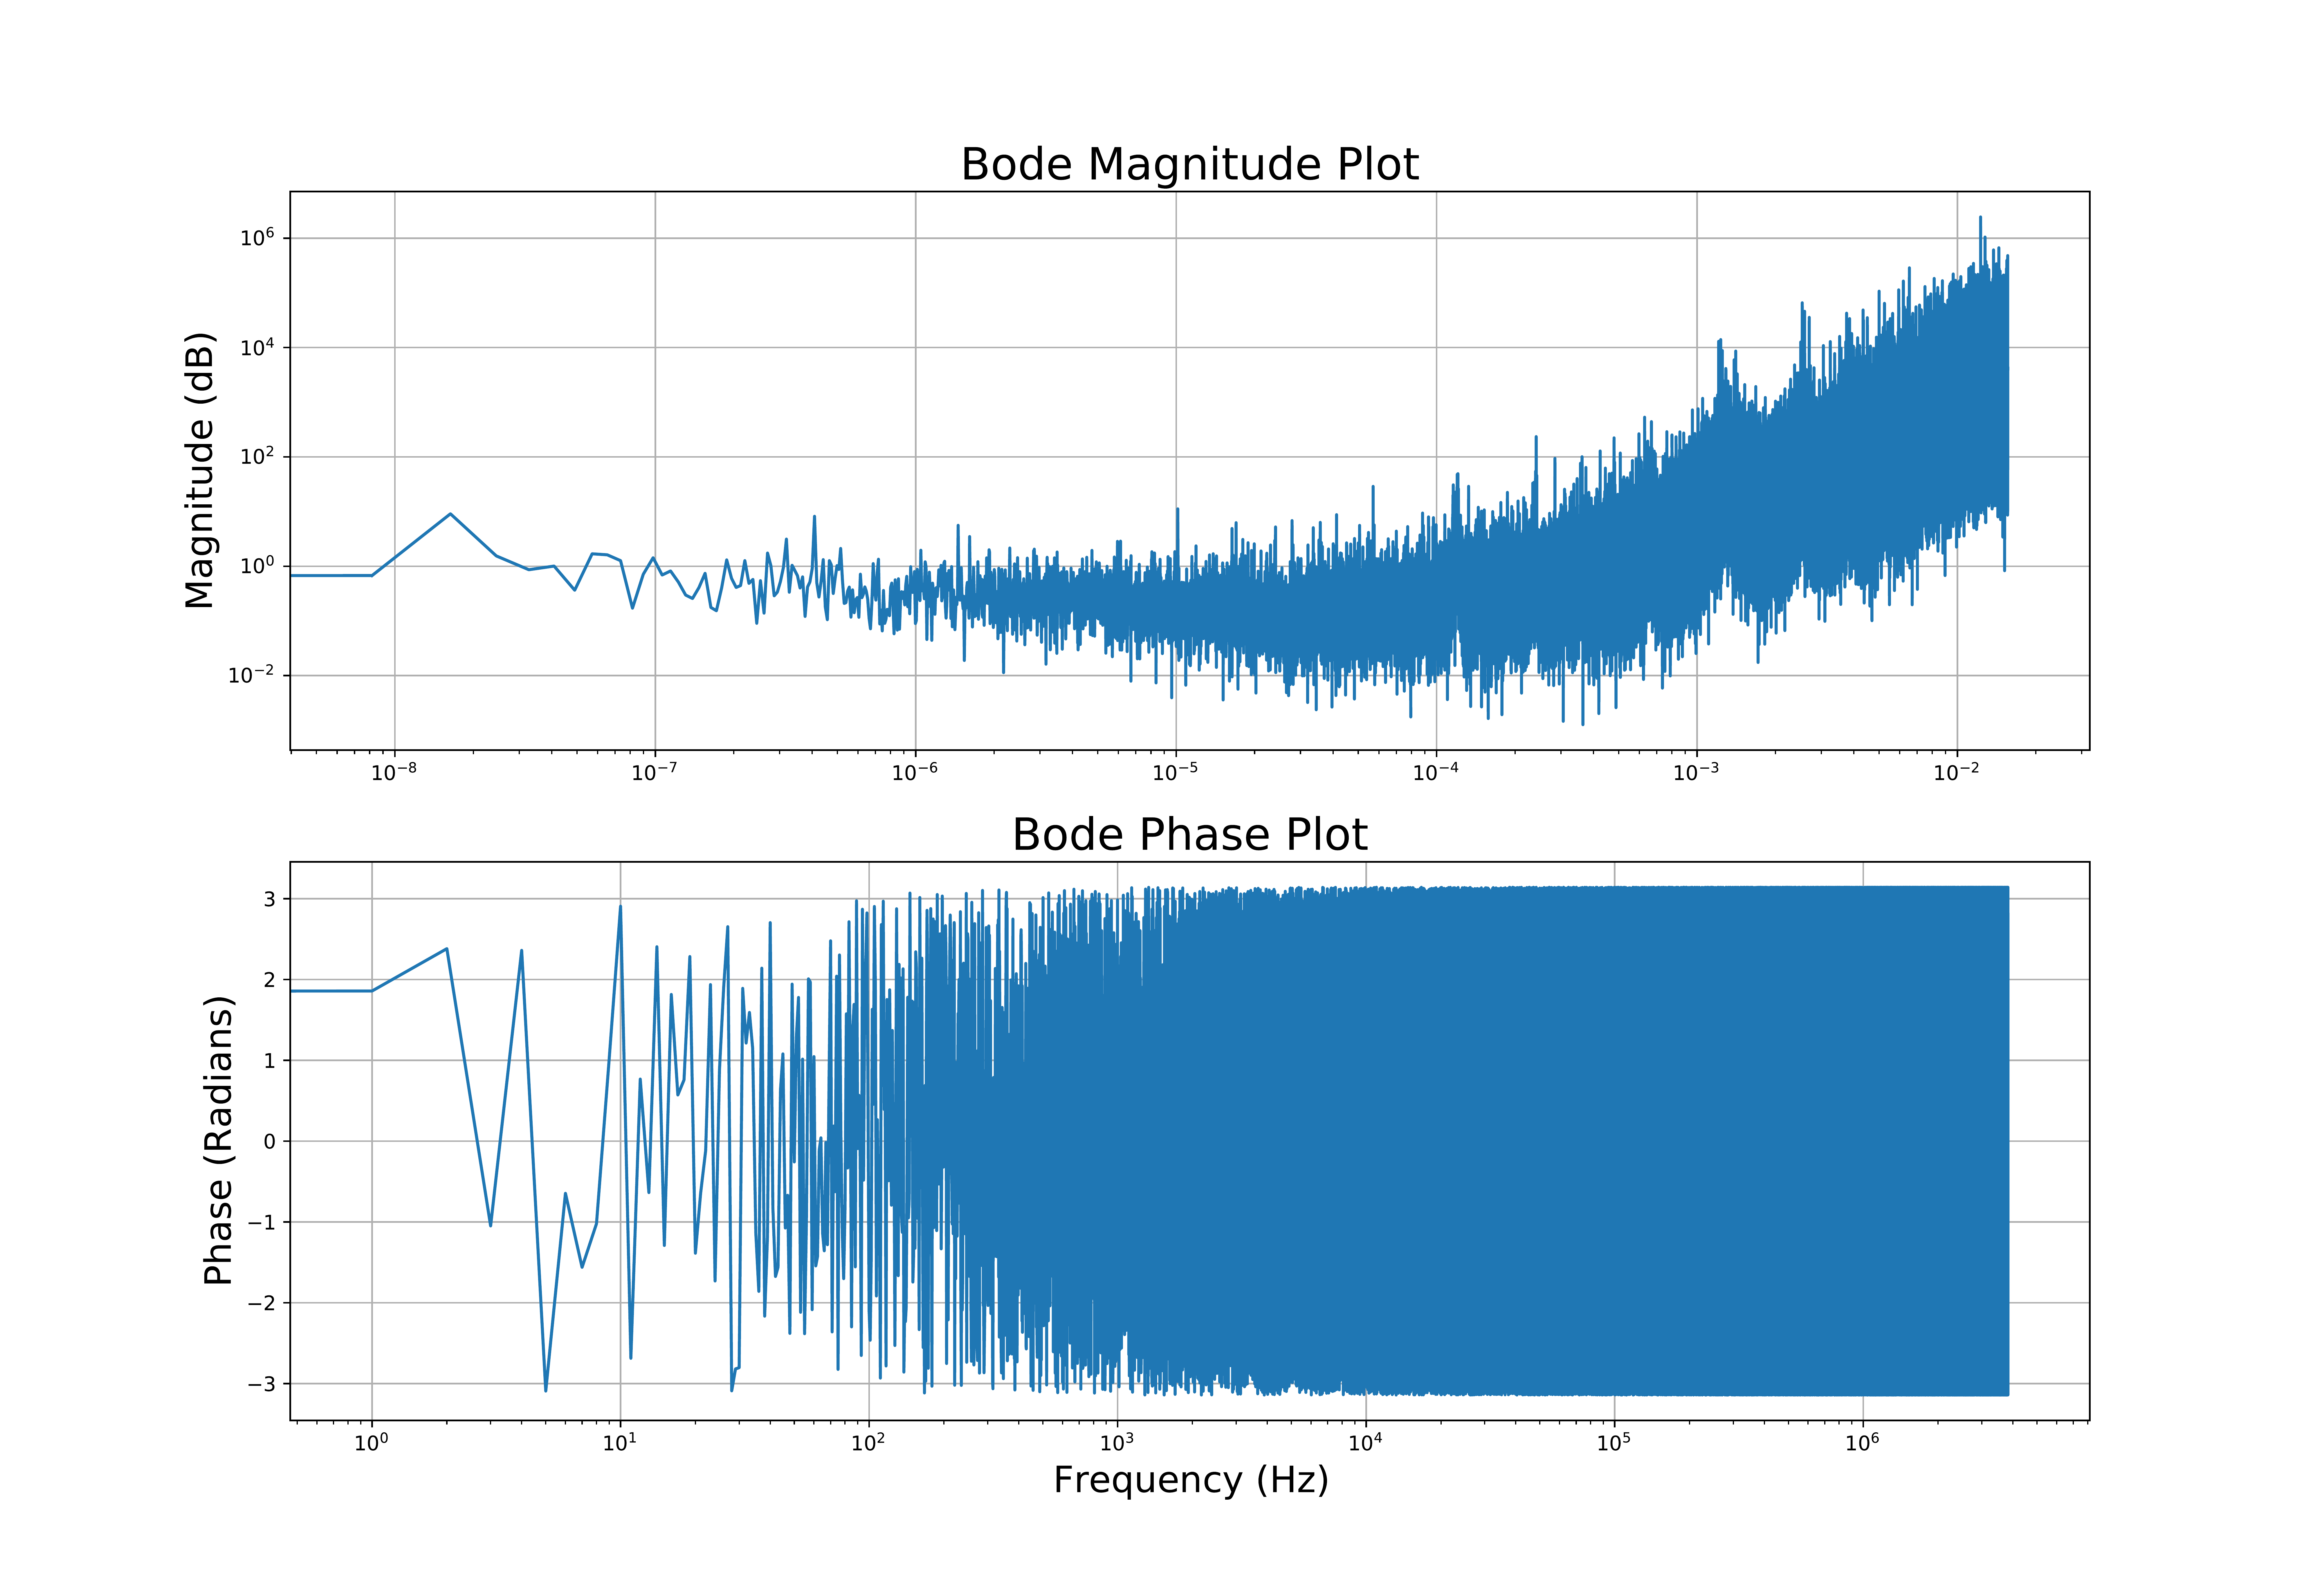
\includegraphics[height=8cm]{Bode_plot-1.png}
\end{frame}
%------------------------------------------------
\begin{frame}{Coherence}
    \centering
    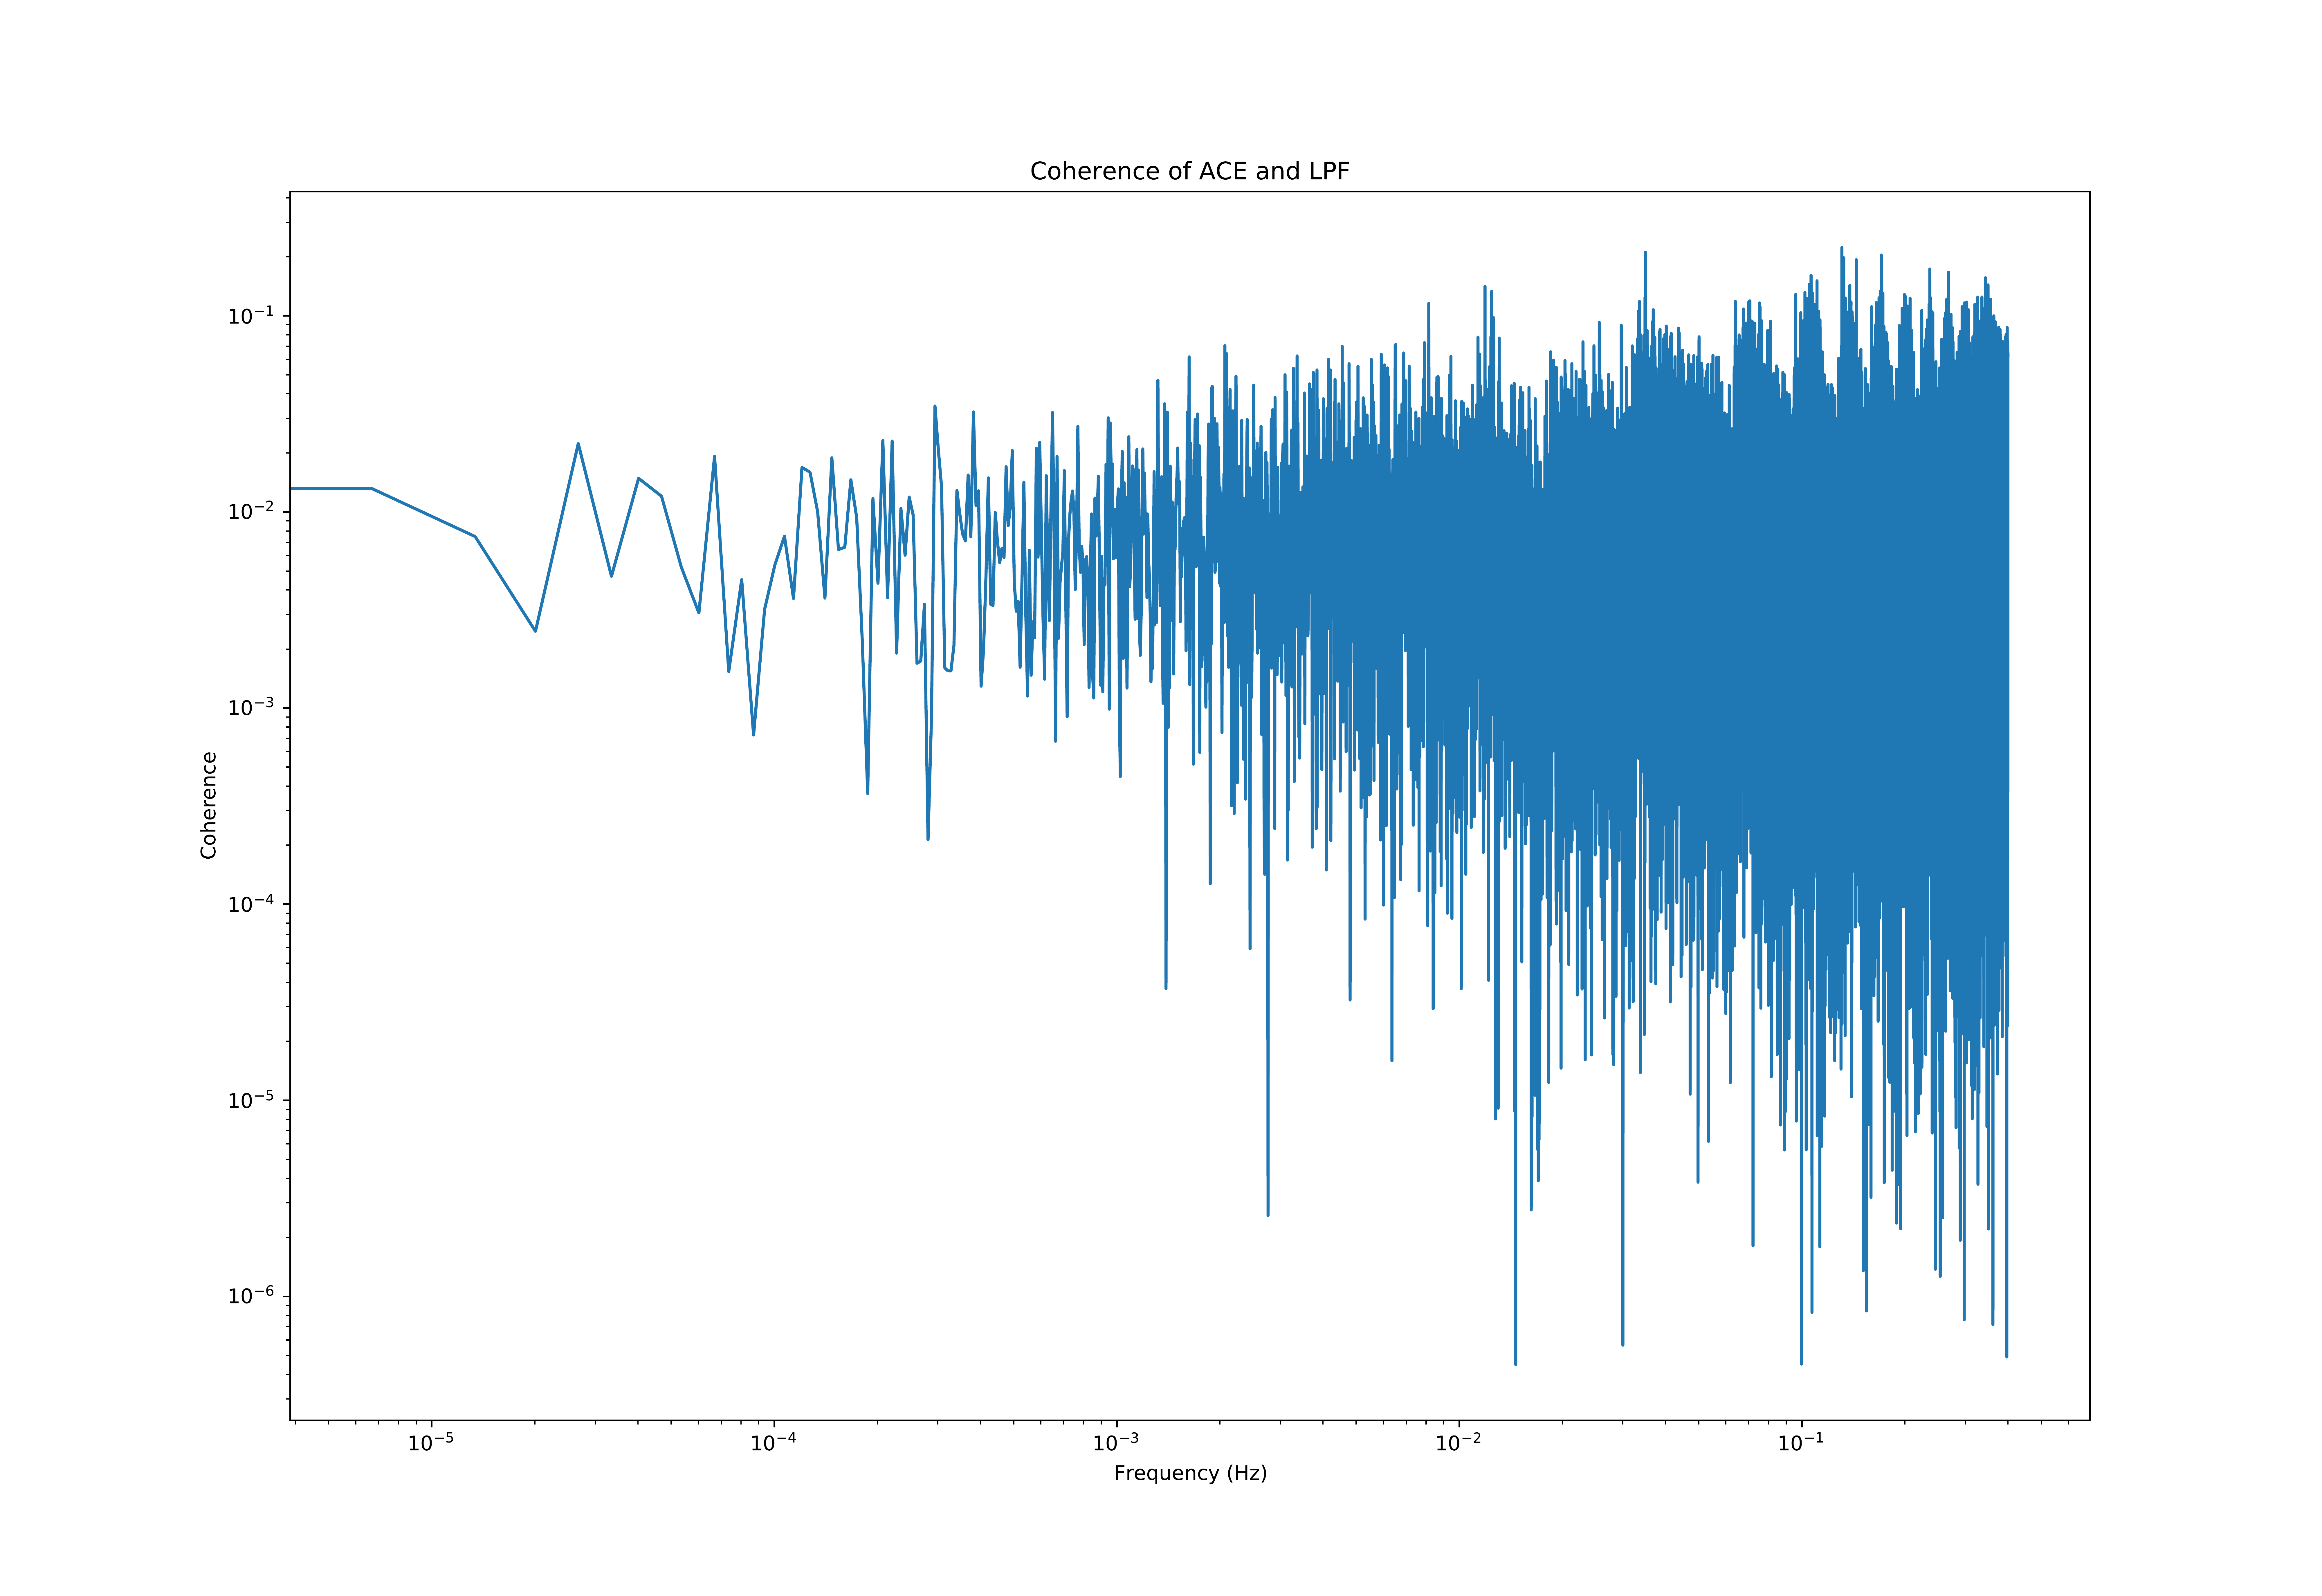
\includegraphics[height=8cm]{ACE_and_LPF_co-1.png}
    \end{frame}
%------------------------------------------------
\begin{frame}{Coherence}
    \centering
    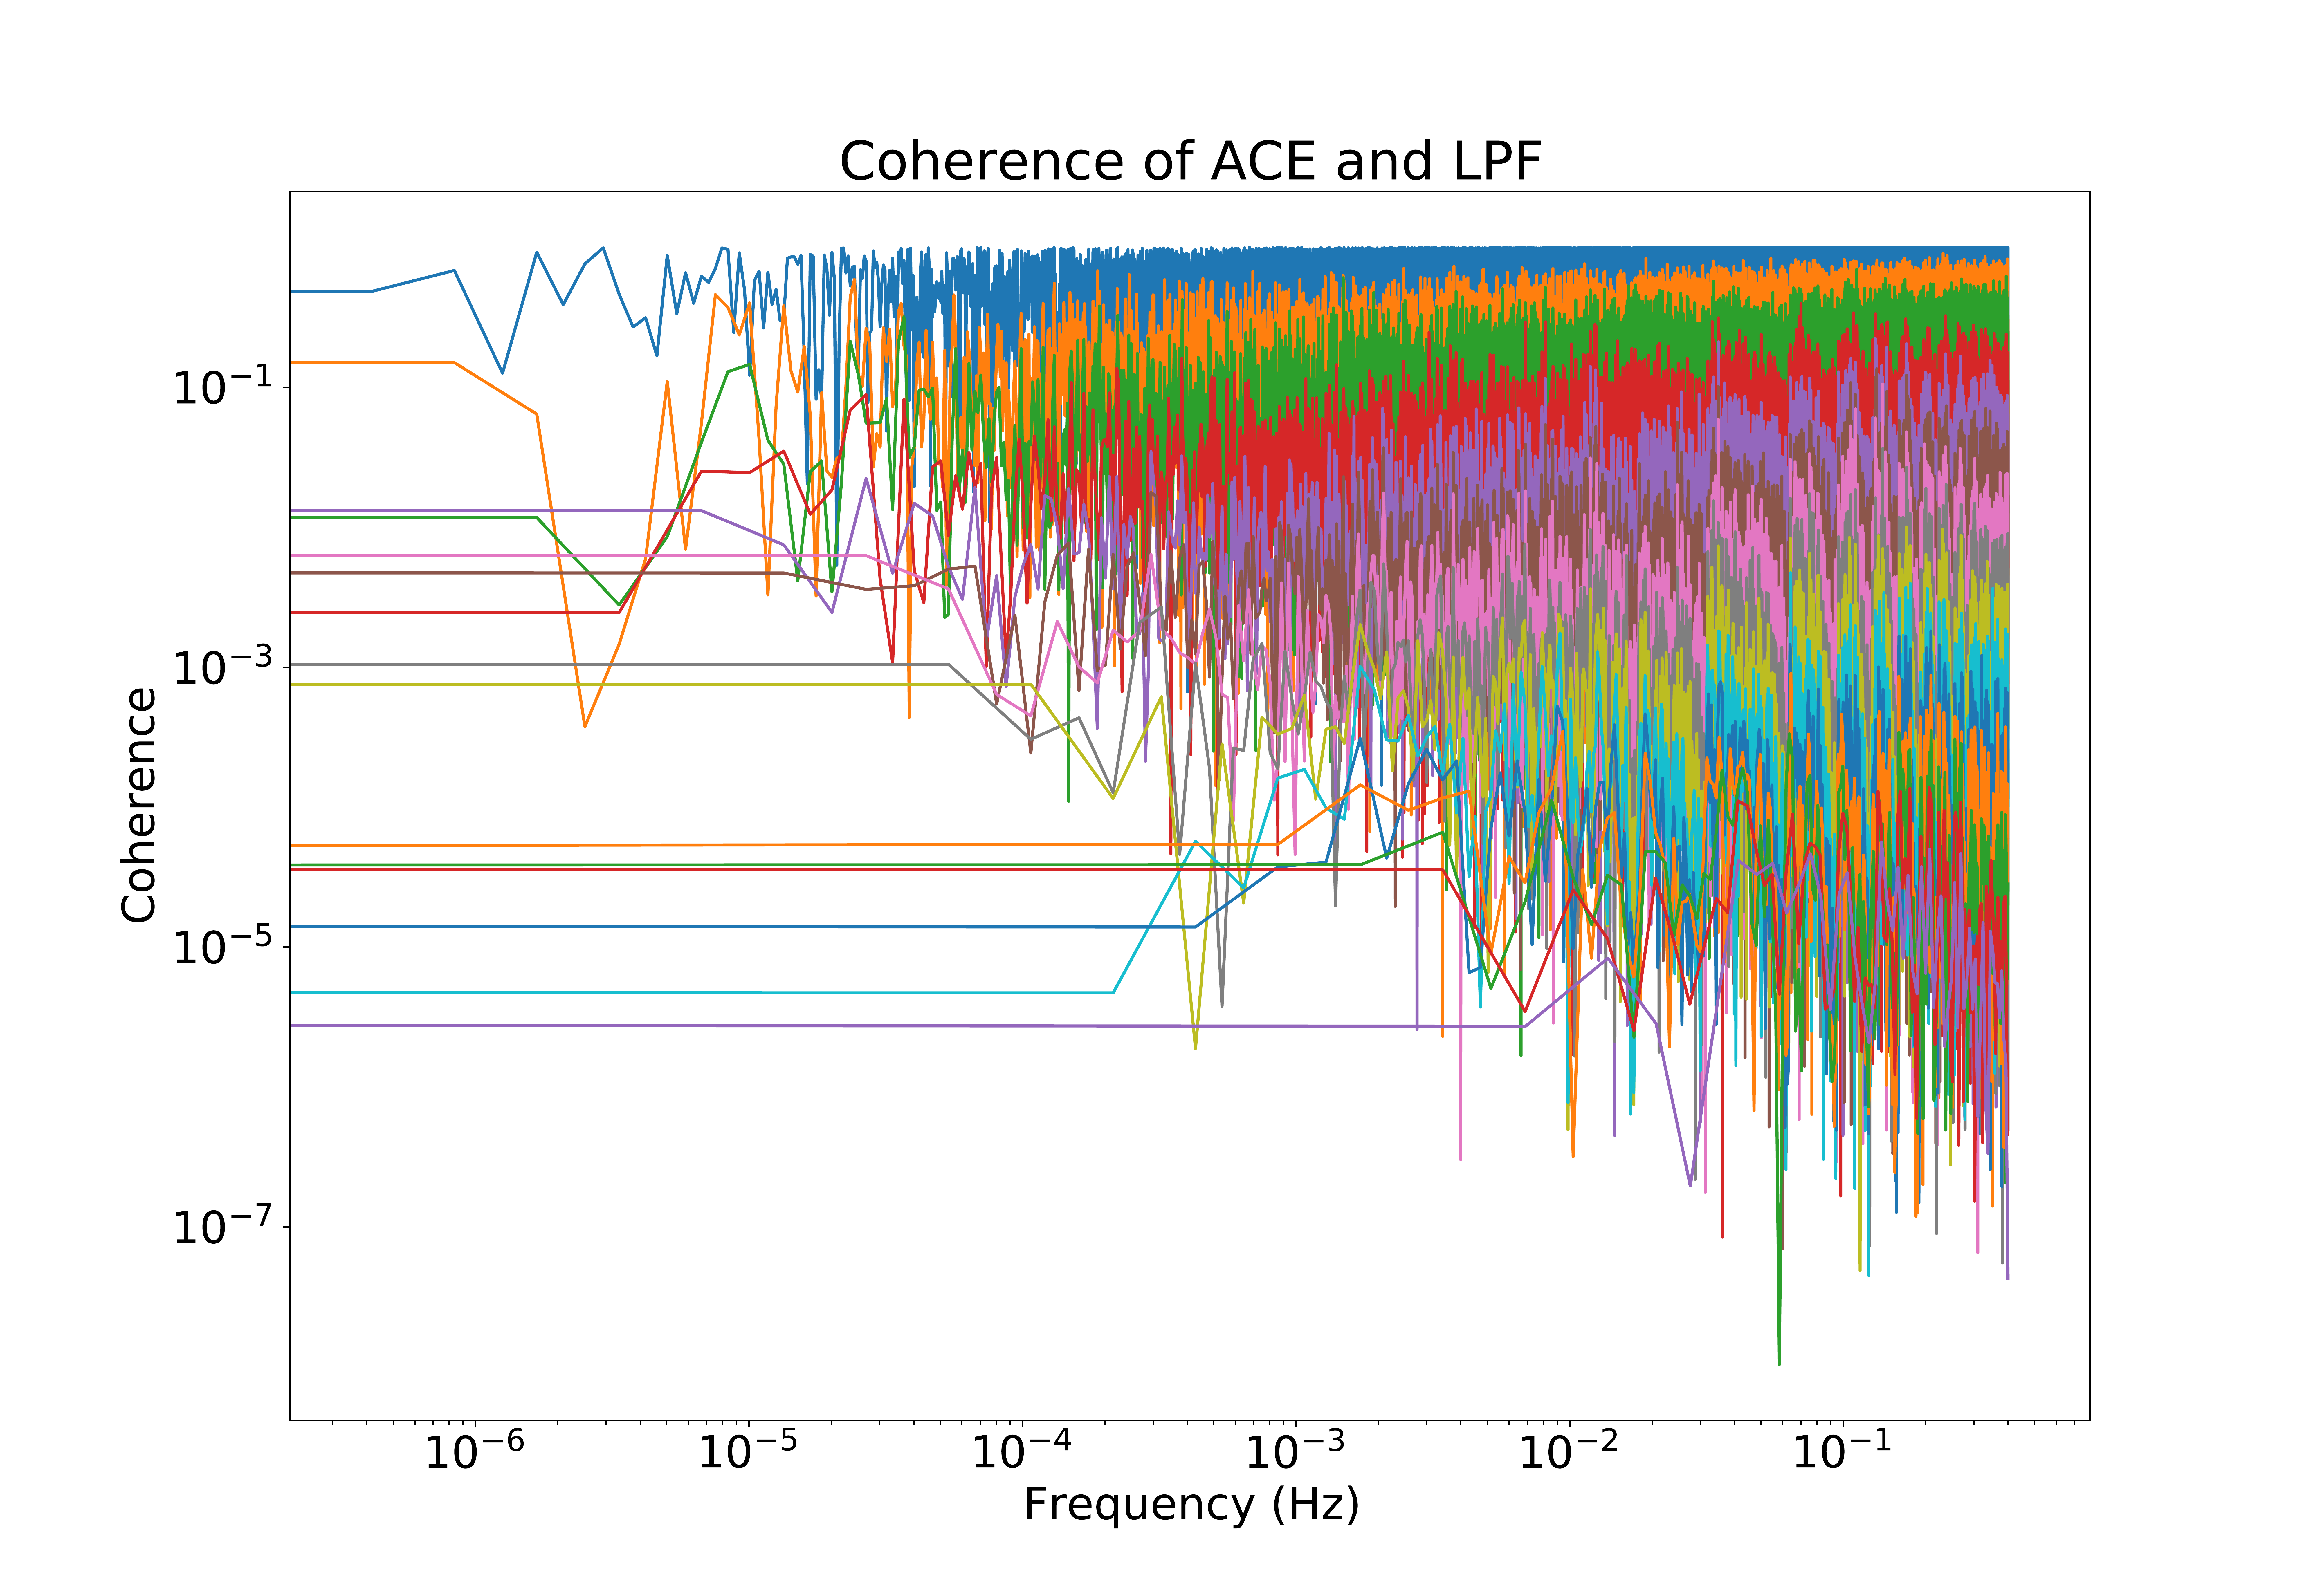
\includegraphics[height=8cm]{ACE_and_LPF_co_2xx15-1.png}
    \end{frame}
%------------------------------------------------
\begin{frame}{Noise Cancellation}
    \centering
    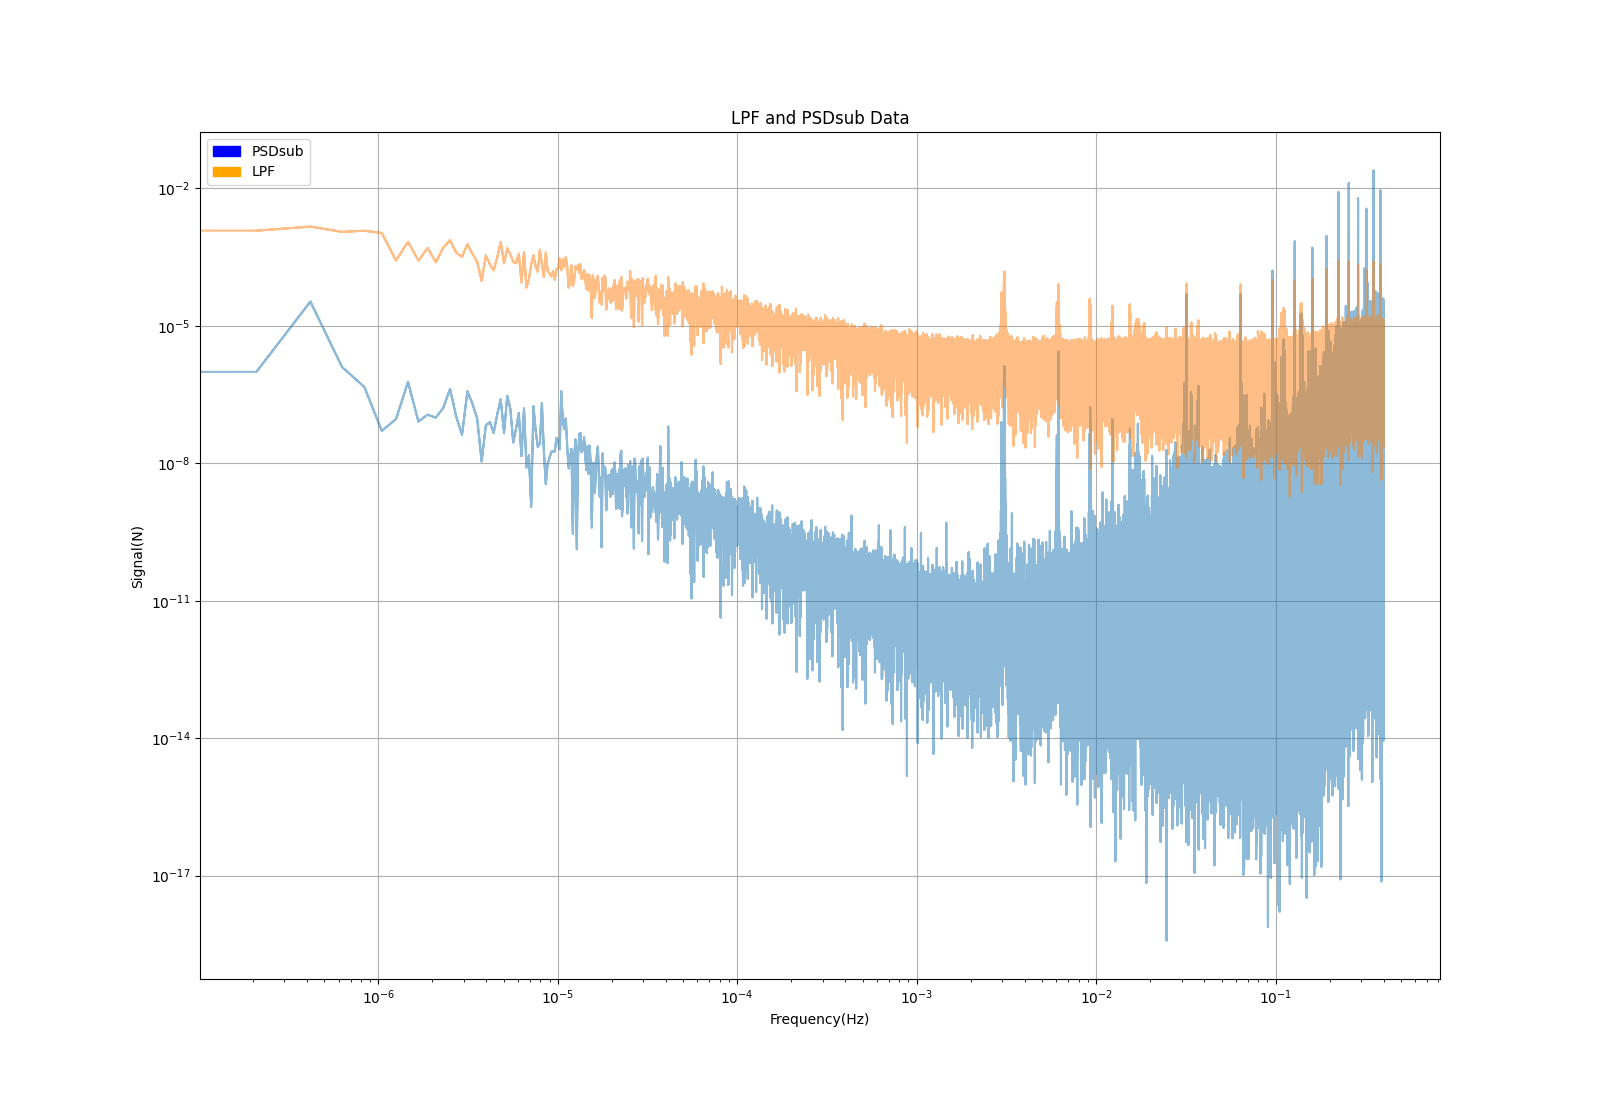
\includegraphics[height=8cm]{LPF_Noise_Cancellation.png}
\end{frame}
%------------------------------------------------
\begin{frame}{Conclusion}
    \large
    \centerline{\textbf{We do not yet measure any significant correlation between ACE solar wind data}}\\
     \centerline{\textbf{ and LISA Pathfinder acceleration noise.}}
\end{frame}
%------------------------------------------------
\begin{frame}{References}
    \centering
    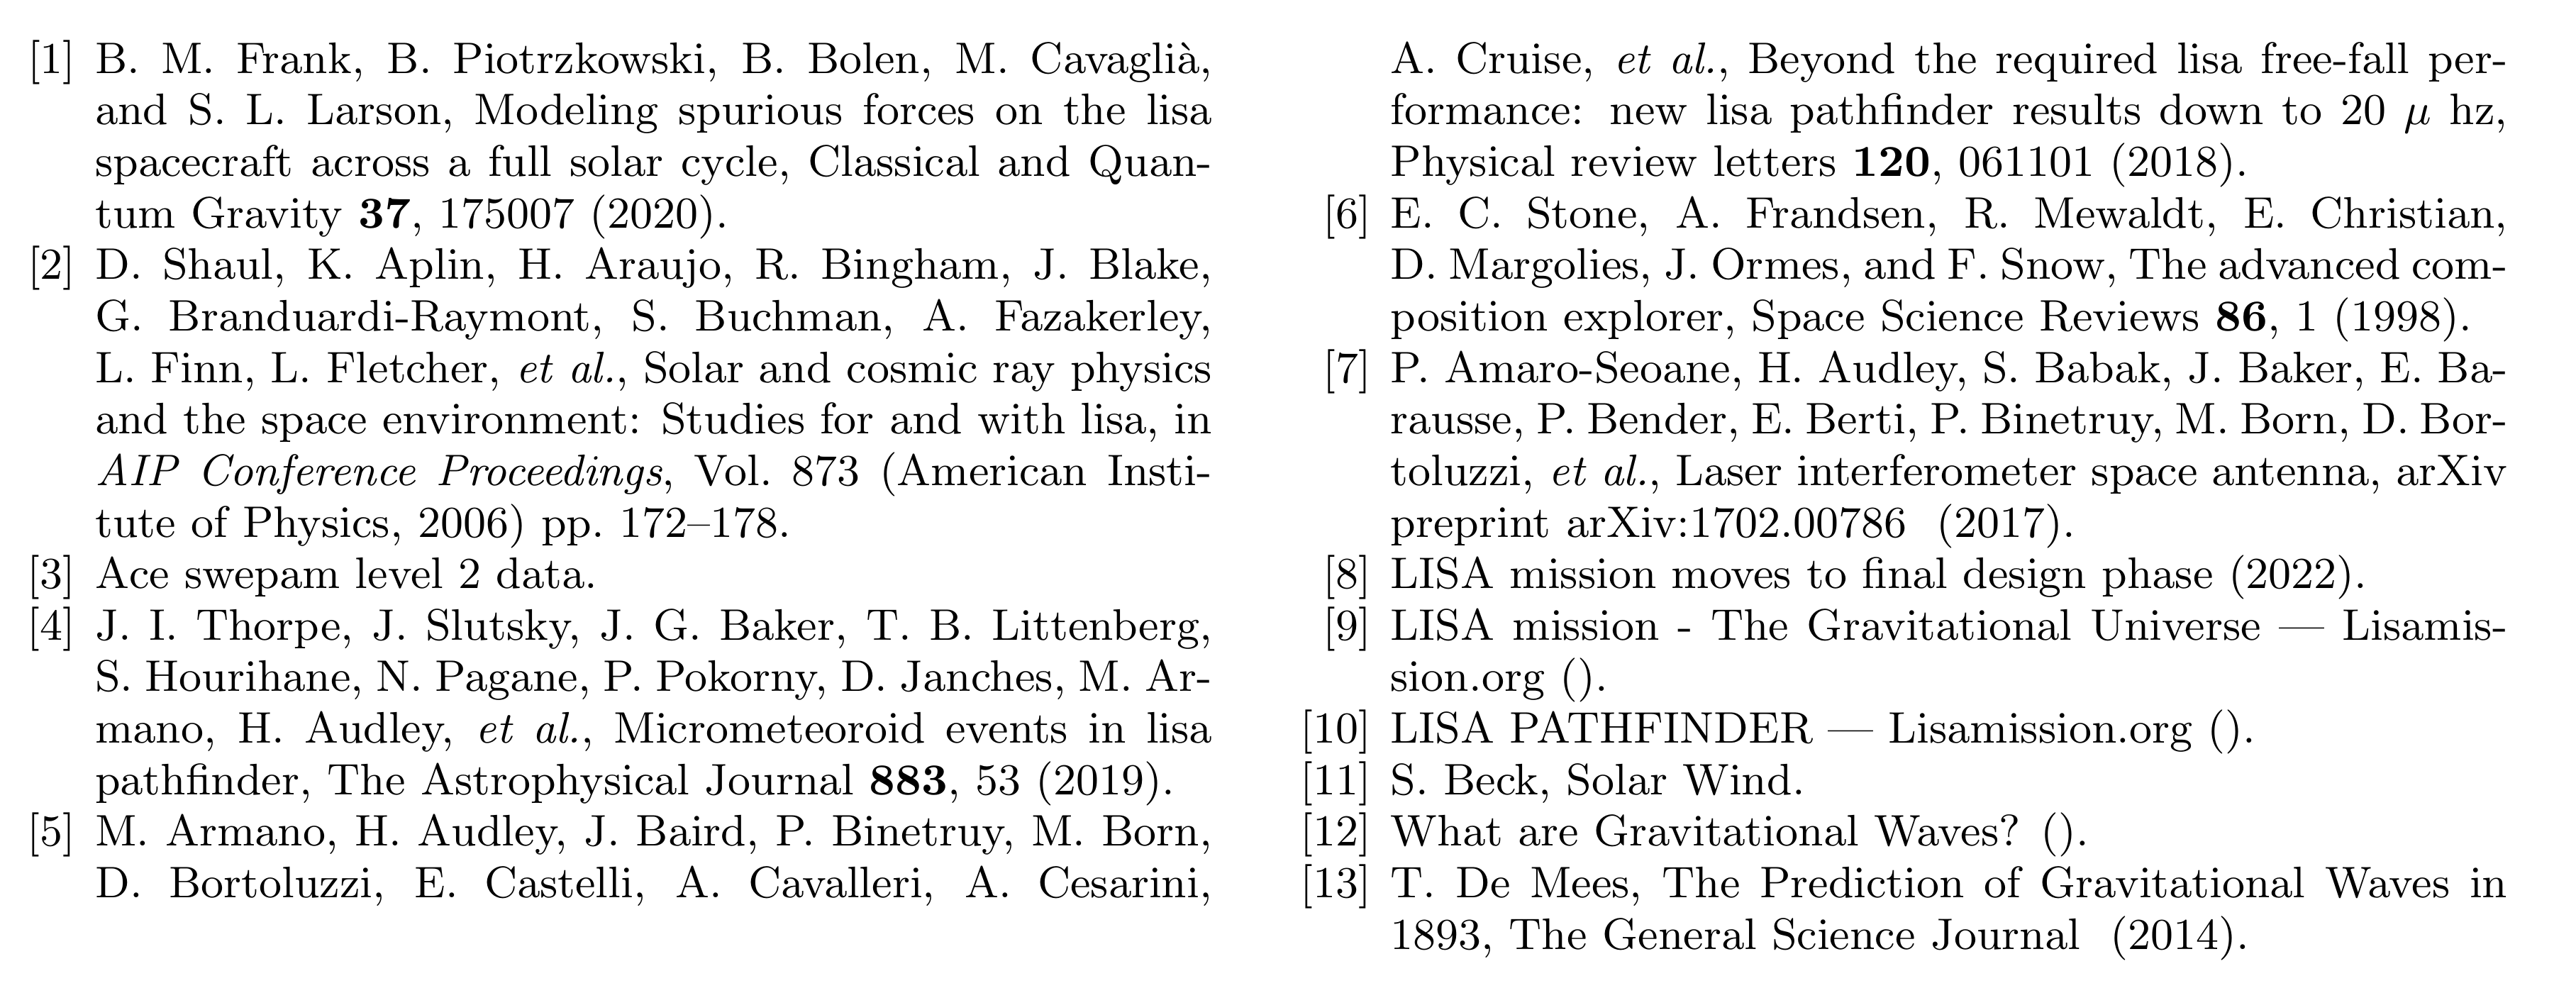
\includegraphics[height=7cm, width=14cm]{bibstuff-1.png}

\end{frame}
%------------------------------------------------

\begin{frame}
    \Huge{\centerline{\textbf{Thank You!!!}}}
\end{frame}
%----------------------------------------------------------------------------------------

\end{document}